% !TeX program = xelatex
% =============================================================================
%  DỰ ÁN TỐT NGHIỆP — BÁO CÁO CHÍNH (BẢN OUTLINE SỰ KIỆN)
%  Đề tài: Phân tích Hiệu suất và Dự báo Sản lượng Hệ thống Điện Mặt Trời
%  Nhóm: The Outliers
%  Trường: Cao đẳng FPT Polytechnic — Chuyên ngành Phân tích Dữ liệu
% =============================================================================

\documentclass[12pt, a4paper]{report}

% ======================== PACKAGES CƠ BẢN & FONT ============================
\usepackage{geometry}
\geometry{a4paper, top=2.5cm, bottom=2.5cm, left=3cm, right=2cm, headheight=33pt, footskip=1.1cm}

% --- FONT CHO XELATEX (HỖ TRỢ TIẾNG VIỆT 100% - FORMAL, TỐI GIẢN, HIỆN ĐẠI) ---
\usepackage{fontspec}
\setmainfont{Times New Roman}
\setmonofont{Consolas}

% ======================== MÀU SẮC & CODE LISTINGS ===========================
\usepackage{xcolor}
\usepackage{listings}
% Định nghĩa bảng màu Tableau trích xuất từ main_fixed_01.twb & tableau_theme.json
\definecolor{tblNavy}{HTML}{4E79A7}
\definecolor{tblOrange}{HTML}{F28E2B}
\definecolor{tblGreen}{HTML}{59A14F}
\definecolor{tblRed}{HTML}{E15759}
\definecolor{tblTeal}{HTML}{76B7B2}
\definecolor{tblYellow}{HTML}{EDC948}
\definecolor{tblPurple}{HTML}{B07AA1}
\definecolor{tblGray}{HTML}{79706E}
\definecolor{tblSeqWarm}{HTML}{F28E2B}


% Định nghĩa màu sắc cho Code Block
\definecolor{mutedgreen}{rgb}{0.2,0.5,0.3} 
\definecolor{mutedblue}{rgb}{0.15,0.35,0.6} 
\definecolor{mutedgray}{rgb}{0.45,0.45,0.45} 
\definecolor{mutedpurple}{rgb}{0.45,0.2,0.55} 
\definecolor{softbackground}{rgb}{0.98,0.98,0.98} 
\definecolor{bordergray}{rgb}{0.85,0.85,0.85} 
\definecolor{fptorange}{RGB}{245,130,32}

\lstdefinestyle{pythonstyle}{
    backgroundcolor   = \color{softbackground},
    commentstyle      = \color{mutedgreen}\itshape,
    keywordstyle      = \color{mutedblue}\bfseries,
    numberstyle       = \tiny\color{mutedgray},
    stringstyle       = \color{mutedpurple},
    basicstyle        = \ttfamily\small\color{black},
    breakatwhitespace = false,
    breaklines        = true,
    captionpos        = t, 
    keepspaces        = true,
    numbers           = left,
    numbersep         = 5pt,
    showspaces        = false,
    showstringspaces  = false,
    showtabs          = false,
    tabsize           = 4,
    frame             = single,
    rulecolor         = \color{bordergray}
}
\lstset{style=pythonstyle}

% Ngăn chặn tự động gạch nối từ (hyphenation) cuối dòng
\hyphenpenalty=10000
\exhyphenpenalty=10000
\tolerance=10000
\emergencystretch=3em

% ======================== TRANG TRÍ & ĐỊNH DẠNG =============================
\usepackage{fancyhdr}
\usepackage{lastpage}
\usepackage{amsmath, amssymb}
\usepackage{enumitem}
\usepackage{array}
\usepackage{booktabs}
\usepackage{tabularx}
\usepackage{longtable}
\usepackage{multirow}
\usepackage{graphicx}
\usepackage{float}
\usepackage{caption}
\usepackage{subcaption}
\usepackage{tikz}
\usepackage[titles]{tocloft}

\usepackage{indentfirst}
\setlength{\parindent}{1cm}
\setlength{\parskip}{6pt}

\usepackage{setspace}
\onehalfspacing
\setlength{\headheight}{33pt}

% Hyperlinks & Bookmarks
\usepackage{hyperref}
\hypersetup{
    colorlinks  = true,
    linkcolor   = black,
    citecolor   = blue,
    filecolor   = magenta,
    urlcolor    = blue,
    pdftitle    = {Dự án Tốt nghiệp - Phân tích Hiệu suất và Dự báo Sản lượng Hệ thống Điện Mặt Trời},
    pdfauthor   = {The Outliers - FPT Polytechnic},
    bookmarksnumbered = true,
}

% --- CẤU HÌNH TIÊU ĐỀ CHƯƠNG ---
\usepackage{titlesec}
\titleformat*{\section}{\fontsize{13pt}{15.6pt}\bfseries}
\titleformat*{\subsection}{\fontsize{13pt}{15.6pt}\bfseries}
\titleformat*{\subsubsection}{\fontsize{13pt}{15.6pt}\bfseries}
\titleformat{\chapter}[display]
  {\normalfont\huge\bfseries}{}{0pt}{\huge}
\titlespacing*{\chapter}{0pt}{-10pt}{20pt} 

% ======================== HEADER / FOOTER ====================================
\fancypagestyle{main}{
    \fancyhf{}
    \fancyhead[L]{
\includegraphics[height=1cm]{figures/logo_fpoly.png}}
    \fancyhead[R]{\small THE OUTLIERS}
    \fancyfoot[L]{\small Dự án Tốt nghiệp}
    \fancyfoot[R]{\small Page \thepage\ of \pageref{LastPage}}
    \renewcommand{\headrulewidth}{0.4pt}
    \renewcommand{\footrulewidth}{0.4pt}
}

\fancypagestyle{plain}{
    \fancyhf{}
    \fancyfoot[L]{\small Dự án Tốt nghiệp}
    \fancyfoot[R]{\small Page \thepage\ of \pageref{LastPage}}
    \renewcommand{\headrulewidth}{0pt}
    \renewcommand{\footrulewidth}{0.4pt}
}

\fancypagestyle{front}{
    \fancyhf{}
    \fancyfoot[L]{\small Dự án Tốt nghiệp}
    \fancyfoot[R]{\small Page \thepage\ of \pageref{LastPage}}
    \renewcommand{\headrulewidth}{0pt}
    \renewcommand{\footrulewidth}{0.4pt}
}

\begin{document}

% ────────────────────────────────────────────────────────────────────
%  TRANG BÌA (COVER PAGE)
% ────────────────────────────────────────────────────────────────────
\begin{titlepage}
\enlargethispage{1.2cm} % SỬA ĐỔI: Chỉ nới rộng tối đa 1.2cm để giữ chữ luôn nằm TRONG khung TikZ

\begin{tikzpicture}[remember picture, overlay]
    \draw[line width=2pt, fptorange]
        ([shift={(1cm,-1cm)}]current page.north west)
        rectangle
        ([shift={(-1cm,1cm)}]current page.south east);
    \draw[line width=0.5pt, fptorange]
        ([shift={(1.15cm,-1.15cm)}]current page.north west)
        rectangle
        ([shift={(-1.15cm,1.15cm)}]current page.south east);
\end{tikzpicture}

\begin{center}
    \textbf{\large TRƯỜNG CAO ĐẲNG FPT POLYTECHNIC}

    \vspace{0.5cm} % Thu nhỏ khoảng cách dưới tên trường
    % --- Logo trường Cao đẳng FPT Polytechnic ---
    
\includegraphics[width=0.38\textwidth]{figures/logo_fpoly.png}

    \vspace{0.4cm}
    {\Large \textbf{DỰ ÁN TỐT NGHIỆP}} \\[4pt]
    {\large \textbf{CHUYÊN NGÀNH: XỬ LÝ DỮ LIỆU}}

    \vspace{1.6cm}
    
    \begin{spacing}{1.0}
        {\huge \textbf{PHÂN TÍCH HIỆU SUẤT VÀ \\[4pt] DỰ BÁO SẢN LƯỢNG \\[4pt] HỆ THỐNG ĐIỆN MẶT TRỜI}}
    \end{spacing}

    \vspace{1.8cm} % Thu nhỏ khoảng cách trước khi vào phần thông tin nhóm
    \normalsize
    \begin{flushleft}
        \hspace{2cm} \textbf{Nhóm thực hiện:} The Outliers \\[5pt]
        \hspace{2cm} \textbf{Sinh viên thực hiện:} \\[3pt]
        % Tạo bảng phụ có chiều rộng cố định (12.5cm) để căn lề MSSV thẳng hàng bên phải
        \hspace{2cm}
        \begin{tabular*}{7.5cm}{@{} l @{\extracolsep{\fill}} r @{}}
            \hspace{0.5cm} 1. Nguyễn Vũ Nhựt   & PS44442 \\
            \hspace{0.5cm} 2. Nguyễn Văn Sỹ    & PS43671 \\
            \hspace{0.5cm} 3. Lê Công Toàn    & PS44145 \\
            \hspace{0.5cm} 4. Nguyễn Xuân Hùng & PS44527 \\
            \hspace{0.5cm} 5. Ngô Tấn Đạt     & PS44589 \\
        \end{tabular*} \\[5pt]
        \hspace{2cm} \textbf{Giảng viên hướng dẫn:} Văn Công Khanh
    \end{flushleft}
    \vfill
    {\normalsize \textbf{TP. HỒ CHÍ MINH, THÁNG 6 NĂM 2026}}
    \vspace{0.5cm} % Tạo một khoảng đệm nhỏ an toàn với đường viền dưới
\end{center}
\end{titlepage}

\pagenumbering{arabic}
\pagestyle{front}

% ────────────────────────────────────────────────────────────────────
%  LỜI CẢM ƠN
% ────────────────────────────────────────────────────────────────────
\chapter*{Lời cảm ơn}
\addcontentsline{toc}{chapter}{Lời cảm ơn}

Lời đầu tiên, nhóm tác giả xin bày tỏ lòng biết ơn sâu sắc và chân thành nhất đến Ban Giám hiệu Trường Cao đẳng FPT Polytechnic, cùng toàn thể quý Thầy, Cô thuộc Bộ môn Công nghệ Thông tin và Chuyên ngành Xử lý Dữ liệu đã tận tình truyền đạt những tri thức nền tảng và chuyên sâu về Kho dữ liệu (Data Warehouse), Quy trình ETL, Phân tích Khám phá Dữ liệu (EDA), và Hệ thống Thông minh Doanh nghiệp (Business Intelligence) trong suốt thời gian nhóm học tập và rèn luyện tại trường.

Đặc biệt, nhóm xin gửi lời tri ân sâu sắc nhất đến \textbf{Thầy Văn Công Khanh} -- Giảng viên Hướng dẫn dự án tốt nghiệp. Trong suốt quá trình thực hiện đề tài, Thầy đã luôn dành nhiều tâm huyết định hướng phương pháp luận khoa học, kiên nhẫn chỉ dẫn từ việc kiểm định chất lượng dữ liệu, thiết kế mô hình hóa kho dữ liệu Galaxy Schema, đến tư duy phân tích các giá trị kinh doanh thực tiễn. Những lời phản biện sắc bén, sự động viên kịp thời và những góp ý quý báu của Thầy chính là nguồn động lực to lớn giúp nhóm vượt qua các thử thách kỹ thuật và hoàn thành đồ án tốt nghiệp này theo đúng chuẩn mực phân tích dữ liệu thực tế tại doanh nghiệp.

Nhóm cũng xin gửi lời cảm ơn trân trọng đến quý Thầy, Cô trong Hội đồng phản biện tốt nghiệp đã dành thời gian quý báu đánh giá và đóng góp những ý kiến chuyên môn sâu sắc giúp đề tài ngày càng hoàn thiện hơn.

Sau cùng, chúng con xin gửi lời tri ân sâu sắc đến gia đình, người thân cùng tất cả bạn bè đã luôn là điểm tựa vững chắc, đồng hành và tạo mọi điều kiện thuận lợi nhất để chúng con hoàn thành trọn vẹn đồ án tốt nghiệp này.

Mặc dù nhóm đã nỗ lực hết mình với tinh thần trách nhiệm cao nhất, song do giới hạn về kinh nghiệm thực tế, báo cáo khó tránh khỏi những thiếu sót nhất định. Nhóm rất mong tiếp tục nhận được sự chỉ bảo và đóng góp ý kiến quý báu từ Thầy Văn Công Khanh và quý Thầy, Cô.

\vspace{0.8cm}
\begin{flushright}
    \textit{TP. Hồ Chí Minh, tháng 6 năm 2026} \\
    \textbf{Nhóm sinh viên thực hiện (The Outliers)}
\end{flushright}

\chapter*{Nhận xét của Giảng viên Hướng dẫn}
\addcontentsline{toc}{chapter}{Nhận xét của Giảng viên Hướng dẫn}
\textit{[Nội dung nhận xét và đánh giá của Giảng viên Hướng dẫn đối với kết quả thực hiện dự án của nhóm.]}

\chapter*{Nhận xét của Giảng viên Phản biện}
\addcontentsline{toc}{chapter}{Nhận xét của Giảng viên Phản biện}
\textit{[Nội dung nhận xét và đánh giá của Giảng viên Phản biện tại buổi bảo vệ dự án tốt nghiệp.]}

% ────────────────────────────────────────────────────────────────────
%  TÓM TẮT DỰ ÁN
% ────────────────────────────────────────────────────────────────────
\chapter*{Tóm tắt Dự án}
\addcontentsline{toc}{chapter}{Tóm tắt Dự án}
Dự án tốt nghiệp ``Phân tich Hiệu suất và Dự báo Sản lượng Hệ thống Điện Mặt Trời'' được thực hiện nhằm xây dựng một nền tảng dữ liệu toàn diện (Nền tảng Dữ liệu Toàn diện) phục vụ công tác giám sát, quản trị vận hành và tối ưu hóa tài chính cho các hệ thống năng lượng mặt trời (PV). 

Xuất phát từ bài toán thực tế của các doanh nghiệp vận hành: mặc dù công suất lắp đặt ngày càng mở rộng nhưng hiệu suất thực tế thường bị thất thoát ẩn do điều kiện thời tiết biến đổi, suy giảm nhiệt độ, bám bụi và hỏng hóc thiết bị biến tần (Inverter). Dự án đã thu thập và tích hợp khối dữ liệu lớn gồm $2.731.946$ bản ghi sản lượng 15 phút từ 42 trạm phát tại 4 khuôn viên thuộc Đại học La Trobe (Úc) cùng dữ liệu khí tượng ERA5-Land từ Open-Meteo API.

Nhóm đã xây dựng quy trình ETL tự động hóa bằng Python, thực hiện làm sạch dữ liệu, xử lý các điểm đứt gãy thời gian, áp dụng rào chắn vật lý và mô hình phân lớp lai GMM--IF để lọc sạch nhiễu cảm biến và gắn nhãn 6 mã lý do kỹ thuật. Dữ liệu được mô hình hóa theo kiến trúc Lược đồ Thiên hà (Galaxy Schema) trên PostgreSQL Supabase và tổng hợp thành các Siêu thị dữ liệu (Siêu thị dữ liệu chuyên đề). Hệ thống 3 Dashboard tương tác trên Tableau cung cấp cho Ban Giám đốc, Quản lý Vận hành và Kỹ sư bảo trì cái nhìn sâu sắc về tỷ lệ hiệu suất (PR), sản lượng đặc trưng (Specific Yield), và tổn thất tài chính, qua đó chuyển đổi dữ liệu thô thành các quyết định vận hành bền vững.

% ────────────────────────────────────────────────────────────────────
%  MỤC LỤC & DANH MỤC
% ────────────────────────────────────────────────────────────────────
\tableofcontents
\listoffigures
\listoftables

\chapter*{Danh mục Từ viết tắt}
\addcontentsline{toc}{chapter}{Danh mục Từ viết tắt}
\vspace*{-15pt}

\noindent\hspace*{-6pt}%
    \begin{tabularx}{\textwidth}{@{} l X @{}}
    \toprule
    \textbf{Ký hiệu/Từ viết tắt} & \textbf{Ý nghĩa đầy đủ} \\
    \midrule
    API       & Application Programming Interface (Giao diện lập trình ứng dụng) \\
    BI        & Business Intelligence (Phân tích thông minh doanh nghiệp) \\
    CF        & Capacity Factor (Hệ số công suất trạm phát) \\
    CSDL      & Cơ sở dữ liệu \\
    CT        & Current Transformer (Cảm biến biến dòng đo dòng điện) \\
    DHI       & Diffuse Horizontal Irradiance (Bức xạ tán xạ mặt phẳng ngang) \\
    DNI       & Direct Normal Irradiance (Bức xạ trực xạ pháp tuyến) \\
    DVC       & Data Version Control (Hệ thống quản lý phiên bản dữ liệu) \\
    DWH       & Data Warehouse (Kho dữ liệu doanh nghiệp) \\
    EDA       & Exploratory Data Analysis (Phân tích khám phá dữ liệu) \\
    ETL       & Extract, Transform, Load (Trích xuất, Biến đổi, Nạp dữ liệu) \\
    FK        & Foreign Key (Khóa ngoại) \\
    GHI       & Global Horizontal Irradiance (Bức xạ tổng cộng mặt phẳng ngang) \\
    GMM       & Gaussian Mixture Model (Mô hình hỗn hợp Gauss) \\
    GMM--IF   & Gaussian Mixture Model -- Isolation Forest Hybrid Pipeline \\
    IEA       & International Energy Agency (Cơ quan Năng lượng Quốc tế) \\
    IF        & Isolation Forest (Thuật toán Rừng cô lập) \\
    IQR       & Interquartile Range (Khoảng tứ phân vị) \\
    KPI       & Key Performance Indicator (Chỉ số đo lường hiệu quả cốt lõi) \\
    kWp       & Kilowatt-peak (Công suất đỉnh cực đại tại điều kiện chuẩn) \\
    Loss Rate & Tỷ lệ tổn thất sản lượng/năng lượng (\%) \\
    O\&M      & Operations and Maintenance (Vận hành và Bảo trì) \\
    OLAP      & Online Analytical Processing (Xử lý phân tích trực tuyến) \\
    PK        & Primary Key (Khóa chính) \\
    PR        & Performance Ratio (Hệ số hiệu suất quang điện) \\
    PV        & Photovoltaic (Quang điện - Năng lượng mặt trời) \\
    RLS       & Row-Level Security (Bảo mật cấp dòng) \\
    STC       & Standard Test Conditions (Điều kiện thử nghiệm tiêu chuẩn) \\
    UI/UX     & User Interface / User Experience (Giao diện / Trải nghiệm người dùng) \\
    WMO       & World Meteorological Organization (Tổ chức Khí tượng Thế giới) \\
    \bottomrule
    \end{tabularx}

\newpage
\pagestyle{main}

% ====================================================================
%  CHƯƠNG 1: GIỚI THIỆU DỰ ÁN VÀ BÀI TOÁN KINH DOANH
% ====================================================================
\chapter{Tổng quan Đề tài và Bài toán Dự án}
\label{chap:tongquan}

\section{Bối cảnh Thực tế và Lý do Chọn Đề tài}
\label{sec:lydo}

Trong xu hướng chuyển dịch năng lượng tái tạo toàn cầu nhằm giảm phát thải khí nhà kính và hướng tới mục tiêu Net Zero, năng lượng mặt trời (quang điện -- Photovoltaic, viết tắt là PV) đang khẳng định vai trò là một trong những nguồn năng lượng sạch có tốc độ phát triển mạnh mẽ nhất. Theo báo cáo thường niên của Cơ quan Năng lượng Quốc tế (IEA)~\cite{iea2023pvps}, tổng công suất lắp đặt quang điện trên toàn cầu đã vượt mốc 1.600~GW. Việc ứng dụng các hệ thống điện mặt trời áp mái tại các cơ quan, trường đại học và khu công nghiệp giúp tiết kiệm đáng kể chi phí điện lưới và chủ động nguồn năng lượng xanh tại chỗ.

Tuy nhiên, đặc tính cơ bản của năng lượng mặt trời là \textbf{tính bất định cao và phụ thuộc phi tuyến vào các điều kiện khí tượng} (bức xạ mặt trời, nhiệt độ môi trường, độ che phủ mây và tốc độ gió). Bên cạnh đó, trong quá trình vận hành dài hạn, các hệ thống quang điện luôn đối mặt với hiện tượng suy giảm hiệu suất do nhiệt độ cao, suy thoái thiết bị biến tần (Inverter), bụi bẩn bám trên bề mặt tấm pin hoặc lỗi truyền thông từ các cảm biến đo đạc.

Do đó, hai bài toán nghiệp vụ cốt lõi đặt ra cho các đơn vị quản lý và vận hành trạm điện mặt trời là:
\begin{enumerate}[noitemsep]
    \item \textbf{Phân tích và Đánh giá Hiệu suất Vận hành:} Theo dõi chính xác các chỉ số hiệu quả chuẩn hóa như Hệ số Hiệu suất (Performance Ratio -- PR), Hệ số Công suất (Capacity Factor -- CF), và Năng suất Riêng (Specific Yield); bóc tách các tổn thất năng lượng do điều kiện môi trường hoặc sự cố thiết bị, đồng thời phát hiện sớm các điểm dữ liệu dị thường để phục vụ công tác bảo trì.
    \item \textbf{Dự báo Sản lượng Điện Mặt trời:} Dự báo chính xác sản lượng điện năng theo chu kỳ ngắn hạn dựa trên chuỗi thời gian lịch sử và thông số khí tượng dự báo, giúp đơn vị quản lý chủ động điều phối phụ tải, tối ưu hóa huy động nguồn điện và nâng cao hiệu quả kinh tế.
\end{enumerate}

Xuất phát từ nhu cầu thực tiễn và tính cấp thiết nêu trên, nhóm tác giả lựa chọn đề tài \textbf{``Phân tích Hiệu suất và Dự báo Sản lượng Hệ thống Điện Mặt Trời''} làm đồ án tốt nghiệp chuyên ngành Xử lý Dữ liệu tại Trường Cao đẳng FPT Polytechnic.

\section{Thực trạng và Thách thức trong Xử lý Dữ liệu Năng lượng Mặt trời}
\label{sec:thuctrang_thachthuc}

Dự án tiếp cận và khai thác nguồn dữ liệu vận hành thực tế quy mô lớn từ bộ dữ liệu mở UNISOLAR của Đại học La Trobe, Úc~\cite{wimalaratne2022unisolar}, kết hợp cùng dữ liệu khí tượng viễn thám ERA5-Land từ Open-Meteo API~\cite{openmeteo2023}. Qua quá trình khảo sát ban đầu, nhóm nghiên cứu đã xác định 4 thách thức kỹ thuật dữ liệu trọng yếu:

\begin{itemize}[noitemsep]
    \item \textbf{Quy mô dữ liệu lớn và Lệch pha độ phân giải thời gian:} Dữ liệu sản lượng gồm hơn $2{,}73$ triệu bản ghi với chu kỳ ghi nhận 15 phút từ 42 trạm phát, trong khi dữ liệu khí tượng viễn thám có chu kỳ 1 giờ. Sự khác biệt về độ chi tiết thời gian đòi hỏi một quy trình xử lý dữ liệu chuẩn hóa và kiến trúc kho dữ liệu đa chiều để tích hợp dữ liệu nhất quán mà không làm phình to dung lượng lưu trữ.
    \item \textbf{Hiện tượng gián đoạn chuỗi thời gian:} Dữ liệu thực tế phát sinh từ cảm biến IoT thường xuất hiện các điểm đứt gãy gián đoạn chu kỳ do lỗi đường truyền mạng. Nếu không được tái lấy mẫu và điền khuyết thời gian một cách khoa học, các tính toán về độ trễ và cửa sổ trượt trong mô hình dự báo chuỗi thời gian sẽ bị sai lệch nghiêm trọng.
    \item \textbf{Nhiễu cảm biến và Dữ liệu dị thường phức tạp:} Sự xuất hiện của các giá trị dòng rò ban đêm khi không có ánh sáng mặt trời do trôi điểm 0 cảm biến, các giá trị phát đột biến vượt công suất thiết kế, hoặc hiện tượng mất phát điện giữa trưa do biến tần ngắt mạch khiến các phương pháp lọc thống kê đơn giản dễ bị sai lệch hoặc loại bỏ nhầm dữ liệu hợp lệ trong những ngày nhiều mây.
    \item \textbf{Nhu cầu Trực quan hóa Quản trị Đa chiều và Dự báo Đáng tin cậy:} Các nhà quản lý vận hành cần một hệ thống bảng điều khiển trực quan tương tác (Dashboard) để theo dõi các chỉ số KPI vận hành và chẩn đoán nguyên nhân sự cố kỹ thuật, song song với một mô hình học máy dự báo sản lượng có độ chính xác cao và khả năng giải thích rõ ràng.
\end{itemize}

\section{Mục tiêu và Nhiệm vụ của Dự án}
\label{sec:muctieu_nhiemvu}

\subsection{Mục tiêu Tổng quát}
Xây dựng một nền tảng kỹ thuật xử lý dữ liệu hoàn chỉnh từ đầu đến cuối nhằm phục vụ công tác giám sát, phân tích hiệu suất vận hành và dự báo sản lượng cho hệ thống điện mặt trời đa trạm phát.

\subsection{Mục tiêu và Nhiệm vụ Cụ thể}
Để hoàn thành mục tiêu tổng quát, dự án tập trung giải quyết 4 nhóm nhiệm vụ chuyên môn:
\begin{enumerate}[label=\arabic*., leftmargin=*]
    \item \textbf{Thu thập, Tiền xử lý và Mô hình hóa Kho Dữ liệu (Kỹ thuật Dữ liệu):}
    \begin{itemize}[noitemsep]
        \item Xây dựng quy trình xử lý dữ liệu tự động (ETL Pipeline) bằng ngôn ngữ Python theo kiến trúc mô-đun độc lập.
        \item Xử lý các điểm gián đoạn thời gian bằng kỹ thuật tái lấy mẫu và điền khuyết chuỗi thời gian liên tục.
        \item Thiết kế và triển khai Kho dữ liệu trung tâm (Data Warehouse) trên nền tảng Supabase theo mô hình Lược đồ Thiên hà (Galaxy Schema) gồm các bảng sự kiện (Fact) và các bảng chiều dữ liệu dùng chung (Dimension).
        \item Thiết lập các cơ chế kiểm tra toàn vẹn dữ liệu và phân quyền bảo mật cấp dòng (RLS).
    \end{itemize}
    \item \textbf{Phát hiện Dị thường và Làm sạch Dữ liệu Nâng cao:}
    \begin{itemize}[noitemsep]
        \item Kết hợp các rào chắn giới hạn vật lý quang điện và mô hình phân lớp lai GMM--IF (Gaussian Mixture Model -- Isolation Forest) để nhận diện chính xác dữ liệu ngoại lai.
        \item Phân loại và gán nhãn các mã lý do kỹ thuật chuẩn hóa phục vụ công tác chẩn đoán và lập kế hoạch bảo trì thiết bị vận hành.
    \end{itemize}
    \item \textbf{Phân tích Khám phá Dữ liệu và Xây dựng Bảng điều khiển Quản trị:}
    \begin{itemize}[noitemsep]
        \item Xây dựng các bảng siêu thị dữ liệu (Data Marts) tính toán trước các chỉ số KPI theo ngày, tháng, trạm phát nhằm tối ưu hóa hiệu năng truy vấn.
        \item Thiết kế hệ thống bảng điều khiển trực quan tương tác trên Tableau Dashboard phục vụ nhu cầu quản lý từ Ban Giám đốc đến Kỹ sư vận hành hiện trường.
    \end{itemize}
    \item \textbf{Mô hình hóa và Dự báo Sản lượng Chuỗi Thời gian:}
    \begin{itemize}[noitemsep]
        \item Xây dựng luồng huấn luyện chuỗi thời gian với kỹ thuật cửa sổ trượt (TimeSeriesSplit), trích xuất đặc trưng chu kỳ tuần hoàn và ngữ cảnh dữ liệu lịch sử.
        \item Thử nghiệm, so sánh các mô hình đường cơ sở (Baseline) và các mô hình học máy tăng cường độ dốc (Gradient Boosting).
        \item Đánh giá mô hình theo các thang đo chuẩn quốc tế và phân tích tầm quan trọng của các yếu tố khí tượng ảnh hưởng đến sản lượng thông qua SHAP.
    \end{itemize}
\end{enumerate}

\section{Đối tượng và Phạm vi Nghiên cứu}
\label{sec:phamvi}

\begin{itemize}[noitemsep]
    \item \textbf{Đối tượng Nghiên cứu:} Dữ liệu sản lượng điện năng từ các trạm quang điện áp mái và các biến số khí tượng viễn thám có ảnh hưởng trực tiếp đến hiệu suất quang điện (bức xạ mặt trời, nhiệt độ môi trường, độ che phủ mây, tốc độ gió, lượng mưa và thời lượng nắng).
    \item \textbf{Phạm vi Không gian:} 42 trạm phát quang điện áp mái với tổng công suất danh định $2.428\,\text{kWp}$ phân bổ tại 4 khuôn viên của Đại học La Trobe, Bang Victoria, Úc (Bundoora, Bendigo, Albury-Wodonga, Shepparton) thuộc bộ dữ liệu mở UNISOLAR~\cite{wimalaratne2022unisolar}.
    \item \textbf{Phạm vi Thời gian:} Chuỗi dữ liệu lịch sử liên tục trong 28 tháng, từ ngày 01/01/2020 đến ngày 30/04/2022.
\end{itemize}

\begin{table}[H]
\centering
\small
\renewcommand{\arraystretch}{1.25}
\begin{tabularx}{\textwidth}{@{} l l X @{}}
\toprule
\textbf{Thông số Khảo sát} & \textbf{Giá trị Thực tế} & \textbf{Ý nghĩa Nghiệp vụ} \\
\midrule
\textbf{Quy mô bản ghi sản lượng} & 2.731.946 dòng & Dữ liệu chuỗi thời gian sản lượng chu kỳ 15 phút từ 42 trạm PV. \\
\textbf{Thời gian thu thập} & 01/01/2020 -- 30/04/2022 & 28 tháng liên tục (bao gồm đủ các mùa khí hậu trong năm). \\
\textbf{Số lượng trạm phát PV} & 42 trạm quang điện áp mái & Quy mô công suất từ trạm nhỏ 10 kWp đến trạm lớn 500 kWp. \\
\textbf{Tổng công suất thiết kế} & 2.428 kWp & Đa dạng các dòng biến tần và cấu hình lắp đặt tấm pin. \\
\textbf{Địa điểm khảo sát} & 4 khuôn viên (Victoria, Úc) & Bundoora, Bendigo, Albury-Wodonga, Shepparton. \\
\textbf{Số biến khí tượng tích hợp} & 8 biến đo lường chuẩn WMO & Bức xạ, nhiệt độ không khí, độ che phủ mây, gió, mưa, nắng. \\
\bottomrule
\end{tabularx}
\caption{Bảng tổng quan thông số dữ liệu thực nghiệm sử dụng trong dự án.}
\label{tab:dataset_summary}
\end{table}

\section{Ý nghĩa Khoa học và Giá trị Ứng dụng Thực tiễn}
\label{sec:ynghia}

\begin{itemize}[noitemsep]
    \item \textbf{Giá trị Kỹ thuật và Học thuật:} Cung cấp một quy trình thực tiễn chuẩn hóa về kỹ thuật xử lý dữ liệu năng lượng tái tạo, giải quyết bài toán tích hợp dữ liệu lệch pha thời gian bằng mô hình Lược đồ Thiên hà và ứng dụng học máy phân lớp lai để phát hiện dữ liệu bất thường.
    \item \textbf{Giá trị Quản trị và Vận hành Doanh nghiệp:} Hệ thống bảng điều khiển trực quan giúp các nhà quản lý nắm bắt toàn diện hiệu suất hệ thống, so sánh hiệu quả giữa các trạm phát, và cung cấp thông tin kịp thời để kỹ sư lên kế hoạch bảo trì.
    \item \textbf{Giá trị Điều độ và Lập kế hoạch Năng lượng:} Các mô hình dự báo chuỗi thời gian hỗ trợ dự đoán chính xác sản lượng phát điện trong ngắn hạn, hỗ trợ việc lập kế hoạch huy động nguồn điện và tối ưu hóa chi phí vận hành.
\end{itemize}

\section{Kế hoạch Thực hiện Dự án (14 Tuần Agile/Scrum)}
\label{sec:kehoach}

Dự án được thực hiện trong thời gian 14 tuần theo phương pháp luận Agile/Scrum với 7 giai đoạn (Sprint) cụ thể:

\begin{table}[H]
\centering
\small
\renewcommand{\arraystretch}{1.25}
\begin{tabularx}{\textwidth}{@{} l l X c @{}}
\toprule
\textbf{Giai đoạn (Sprint)} & \textbf{Thời gian} & \textbf{Hạng mục Công việc Trọng tâm} & \textbf{Trạng thái} \\
\midrule
Sprint 1: Khảo sát \& Phân tích & Tuần 1--2 & Khảo sát dữ liệu 42 trạm UNISOLAR và phân tích khám phá ban đầu. & Hoàn thành \\
Sprint 2: ETL \& Tiền xử lý & Tuần 3--5 & Xây dựng pipeline xử lý dữ liệu tự động, tái lấy mẫu và điền khuyết. & Hoàn thành \\
Sprint 3: Mô hình hóa Kho Dữ liệu & Tuần 6--8 & Thiết kế mô hình Lược đồ Thiên hà và nạp dữ liệu vào Supabase DWH. & Hoàn thành \\
Sprint 4: Lọc Dị thường Nâng cao & Tuần 8--10 & Triển khai rào chắn vật lý và mô hình phân lớp lai GMM--IF gán mã lý do. & Hoàn thành \\
Sprint 5: Xây dựng Dashboard & Tuần 10--12 & Xây dựng các siêu thị dữ liệu và hoàn thiện hệ thống Dashboard Tableau. & Hoàn thành \\
Sprint 6: Mô hình Hóa Dự báo & Tuần 12--13 & Huấn luyện, đánh giá và so sánh các mô hình học máy dự báo chuỗi thời gian. & Hoàn thành \\
Sprint 7: Nghiệm thu \& Đóng gói & Tuần 14 & Hoàn thiện báo cáo đồ án, đóng gói mã nguồn và nghiệm thu toàn diện. & Hoàn thành \\
\bottomrule
\end{tabularx}
\caption{Bảng tổng hợp tiến độ thực hiện và kết quả đạt được của dự án qua 14 tuần.}
\label{tab:project_timeline}
\end{table}

\section{Bố cục Báo cáo Đồ án Tốt nghiệp}
\label{sec:bocuc}

Báo cáo dự án tốt nghiệp được cấu trúc thành 7 chương liền mạch theo đúng quy trình phân tích và xử lý dữ liệu chuẩn:
\begin{itemize}[noitemsep]
    \item \textbf{Chương 1: Tổng quan Đề tài và Bài toán Dự án} -- Trình bày bối cảnh thực tế, lý do chọn đề tài, thách thức dữ liệu, mục tiêu nghiên cứu, phạm vi, ý nghĩa và kế hoạch thực hiện dự án.
    \item \textbf{Chương 2: Cơ sở Lý thuyết và Kiến trúc Hệ thống} -- Trình bày các kiến thức nền tảng về năng lượng mặt trời, bộ chỉ số đo lường hiệu suất (KPI), lý thuyết Kho dữ liệu đa chiều, kiến trúc luồng xử lý dữ liệu và nguyên tắc trực quan hóa.
    \item \textbf{Chương 3: Thu thập, Tiền xử lý và Mô hình hóa Kho Dữ liệu} -- Trình bày chi tiết kiến trúc mô-đun xử lý dữ liệu, kết quả kiểm định chất lượng ban đầu, kỹ thuật trích xuất đặc trưng, và thiết kế mô hình Lược đồ Thiên hà (Galaxy Schema) trên Supabase.
    \item \textbf{Chương 4: Phát hiện Dị thường và Làm sạch Dữ liệu Nâng cao} -- Trình bày thuật toán phân lớp lai GMM--IF kết hợp rào chắn giới hạn vật lý, phân loại các mã lý do dị thường kỹ thuật, và cơ chế đảm bảo tính toàn vẹn dữ liệu.
    \item \textbf{Chương 5: Phân tích Khám phá Dữ liệu và Trực quan hóa Dashboard} -- Trình bày kết quả phân tích khám phá dữ liệu chuyên sâu và thiết kế hệ thống bảng điều khiển trực quan quản trị trên Tableau.
    \item \textbf{Chương 6: Khai phá Dữ liệu và Dự báo Sản lượng} -- Trình bày quy trình tiền xử lý chuỗi thời gian, huấn luyện và đánh giá các mô hình học máy dự báo sản lượng, phân tích tầm quan trọng của đặc trưng bằng SHAP và các phát hiện thực tiễn.
    \item \textbf{Chương 7: Kết luận và Hướng phát triển} -- Tổng kết các kết quả đạt được của đề tài, nêu rõ những hạn chế và đề xuất các giải pháp nâng cấp trong tương lai.
\end{itemize}

% ====================================================================
%  CHƯƠNG 2: CƠ SỞ LÝ THUYẾT VÀ KIẾN TRÚC HỆ THỐNG
% ====================================================================
\chapter{Cơ sở Lý thuyết và Kiến trúc Hệ thống}
\label{chap:lythuyet}

\section{Cơ sở Lý thuyết}
\label{sec:co_so_ly_thuyet}

\subsection{Khái quát về Phân tích Dữ liệu trong Ngành Năng lượng Tái tạo}
Phân tích dữ liệu trong ngành năng lượng mặt trời là quá trình thu thập, làm sạch, mô hình hóa và khai phá thông tin chuyên sâu từ khối lượng lớn chuỗi thời gian sản lượng điện và dữ liệu khí tượng. Trong bối cảnh vận hành các trạm điện mặt trời hiện đại, dữ liệu đóng vai trò là tài sản chiến lược giúp tối ưu hóa hiệu suất phát điện, giảm thiểu chi phí bảo trì và bảo vệ dòng tiền đầu tư.

Theo chuẩn mực phân tích dữ liệu doanh nghiệp, các cấp độ phân tích trong đề tài được phân chia rõ ràng:
\begin{itemize}[noitemsep]
    \item \textbf{Phân tích Mô tả (Phân tích Mô tả):} Trả lời câu hỏi \textit{``Chuyện gì đã xảy ra?''} thông qua việc tổng hợp sản lượng thực tế, tính toán hệ số hiệu suất (PR), hệ số công suất (CF) và năng suất riêng (Specific Yield) của 42 trạm phát qua từng tháng và từng năm.
    \item \textbf{Phân tích Chẩn đoán (Phân tích Chẩn đoán):} Trả lời câu hỏi \textit{``Tại sao hiệu suất trạm lại suy giảm?''} bằng cách bóc tách mối tương quan giữa sản lượng và các yếu tố khí tượng (nhiệt độ quá cao, mây che phủ) hoặc lỗi phần cứng (Inverter ngắt mạch, hỏng diode, trôi cảm biến đo ban đêm).
    \item \textbf{Phân tích Dự báo (Phân tích Dự báo):} Trả lời câu hỏi \textit{``Sản lượng điện trong chu kỳ tiếp theo là bao nhiêu?''} để hỗ trợ đơn vị vận hành lập kế hoạch điều phối phụ tải và huy động nguồn điện dự phòng.
    \item \textbf{Phân tích Đề xuất (Phân tích Đề xuất):} Đưa ra các khuyến nghị bảo trì cụ thể (vệ sinh bề mặt pin, thay thế biến tần quá nhiệt, hiệu chuẩn cảm biến CT).
\end{itemize}

\subsection{Các Chỉ số Hiệu năng Cốt lõi (KPIs) và Bài toán Tổn thất Vận hành}
Trong quản trị vận hành trạm quang điện, tổng sản lượng (kWh) chỉ phản ánh quy mô phát điện thô, trong khi các chỉ số hiệu chuẩn hóa mới là thước đo chính xác về chất lượng vận hành:
\begin{enumerate}[label=\arabic*., leftmargin=*]
    \item \textbf{Hệ số Hiệu suất (Performance Ratio -- PR):} Tỷ số giữa sản lượng điện thực tế tạo ra ($E_{\text{actual}}$) và sản lượng lý thuyết trong điều kiện bức xạ thu nhận được:
    \begin{equation}
        \text{PR} = \frac{E_{\text{actual}}}{P_{\text{stc}} \cdot \left(\frac{GHI}{1000\,\text{W/m}^2}\right) \cdot \Delta t} \times 100\%
    \end{equation}
    Chỉ số PR tiêu chuẩn của hệ thống tốt thường đạt từ $75\%$ đến $85\%$. Khi $\text{PR} < 70\%$, hệ thống đang gặp tổn thất vận hành nghiêm trọng.
    
    \item \textbf{Hệ số Công suất (Capacity Factor -- CF):} Tỷ lệ giữa năng lượng thực tế thu được trong một khoảng thời gian so với năng lượng tối đa nếu trạm phát liên tục ở công suất danh định $24/24\text{h}$:
    \begin{equation}
        \text{CF} = \frac{\sum E_{\text{actual}}}{P_{\text{stc}} \cdot 8760\,\text{h}} \times 100\%
    \end{equation}
    
    \item \textbf{Năng suất Riêng (Specific Yield -- $\text{kWh/kWp}$):} Lượng điện năng tạo ra trên mỗi kWp công suất lắp đặt, là thước đo công bằng nhất để so sánh hiệu quả giữa các trạm có quy mô công suất khác nhau.

    \item \textbf{Hệ số Tổn thất Nhiệt độ (Tổn thất Suy hao do Nhiệt độ):} Khi nhiệt độ môi trường vượt quá $25^\circ\text{C}$ (nhiệt độ cell pin đạt $50-65^\circ\text{C}$), công suất phát bị suy giảm tuyến tính theo hệ số nhiệt độ $\gamma \approx -0{,}35\%/^\circ\text{C}$ đến $-0{,}50\%/^\circ\text{C}$:
    \begin{equation}
        P_{\text{loss, temp}} = P_{\text{stc}} \cdot |\gamma| \cdot (T_{\text{cell}} - 25^\circ\text{C})
    \end{equation}
    
    \item \textbf{Tổn thất Biến tần (Tổn thất Biến tần) theo IEA-PVPS Task 13~\cite{iea2023pvps}:} Biến tần có thời gian trung bình giữa các sự cố (MTBF) ngắn hơn tấm pin $300-500$ lần, gây ra 36\% tổng tổn thất phần cứng của hệ thống.
\end{enumerate}

\subsection{Hệ thống Kho Dữ liệu (Data Warehouse) và Quy trình ETL}
Kho dữ liệu (Data Warehouse -- DWH) là hệ thống cơ sở dữ liệu được thiết kế chuyên biệt để hỗ trợ các hoạt động phân tích thông minh (BI) và báo cáo quản trị (OLAP), phân tách hoàn toàn khỏi các hệ thống xử lý giao dịch vận hành (OLTP).

Để chuyển hóa dữ liệu thô thành thông tin quản trị, quy trình ETL được thực thi theo 3 giai đoạn:
\begin{itemize}[noitemsep]
    \item \textbf{Trích xuất Dữ liệu (Extract):} Thu thập dữ liệu chuỗi thời gian sản lượng từ tệp tin cục bộ và gọi API khí tượng Open-Meteo.
    \item \textbf{Transform (Biến đổi \& Làm sạch):} Chuẩn hóa kiểu dữ liệu, xử lý giá trị khuyết thiếu (Imputation), xử lý đứt gãy thời gian (điểm gián đoạn thời gian), gắn nhãn ngoại lai bằng rào chắn vật lý và trích xuất đặc trưng nghiệp vụ.
    \item \textbf{Nạp Dữ liệu vào Kho (Load):} Nạp dữ liệu có cấu trúc vào kho lưu trữ tập trung Supabase DWH theo mô hình đa chiều.
\end{itemize}

\subsection{Mô hình Dữ liệu Đa chiều và Lược đồ Thiên hà (Galaxy Schema)}
Mô hình đa chiều do Ralph Kimball~\cite{kimball2013dwh} đề xuất phân tách dữ liệu thành:
\begin{itemize}[noitemsep]
    \item \textbf{Bảng sự kiện (Fact Table):} Chứa các chỉ số đo lường định lượng theo chuỗi thời gian như \texttt{fact\_solar\_energy\_gen} (sản lượng điện 15 phút) và \texttt{fact\_weather} (thông số khí tượng 1 giờ).
    \item \textbf{Bảng chiều (Dimension Table):} Chứa các thuộc tính ngữ cảnh mô tả như \texttt{dim\_solar\_plant} (trạm phát), \texttt{dim\_date} (ngày), \texttt{dim\_time} (giờ), \texttt{dim\_weather\_type} (mã thời tiết).
\end{itemize}

Trong dự án này, do dữ liệu sản lượng và dữ liệu thời tiết có tần suất ghi nhận lệch nhau (15 phút vs 1 giờ), nhóm sử dụng \textbf{Lược đồ Thiên hà (Mô hình Lược đồ Thiên hà -- Galaxy Schema)}. Hai bảng Fact độc lập liên kết chặt chẽ với nhau thông qua 4 bảng Dimension dùng chung (chiều dữ liệu dùng chung), đảm bảo không làm phình to dữ liệu và tối ưu hóa hiệu năng truy vấn liên thông (Drill-through).

\subsection{Phương pháp Phát hiện Dị thường và Lọc Nhiễu Nghiệp vụ}
Để đảm bảo nguyên tắc ``Dữ liệu sạch = Insight đúng'', quy trình xử lý dữ liệu tích hợp các phương pháp phát hiện dị thường nhằm phục vụ công tác làm sạch:
\begin{itemize}[noitemsep]
    \item \textbf{Khoảng Tứ phân vị IQR (Tukey 1977~\cite{tukey1977eda}):} Xác định ngưỡng phân vị $\text{IQR} = Q_3 - Q_1$ để loại trừ các giá trị đo đột biến cục bộ.
    \item \textbf{Rào chắn Vật lý (Physical Boundaries):} Thiết lập 5 giới hạn vật lý năng lượng mặt trời (cắt trần công suất danh định, loại bỏ phát điện ban đêm $GHI=0$, phát hiện nắng gắt mất điện).
    \item \textbf{Phân lớp Lai GMM--IF (Li et al., 2025~\cite{li2025gmmif}):} Đóng vai trò như một bộ lọc thông minh trong tầng Transform, phân đoạn dữ liệu thành các vùng lá thời tiết đồng nhất để nhận diện chính xác các điểm dữ liệu dị thường do lỗi thiết bị và gán 6 mã lý do kỹ thuật phục vụ bảo trì.
\end{itemize}

\subsection{Trực quan hóa Dữ liệu trong Business Intelligence (BI)}
Trực quan hóa dữ liệu không đơn thuần là vẽ biểu đồ làm đẹp, mà là công cụ khám phá tri thức kinh doanh (Business Storytelling). Các nguyên tắc thiết kế được tuân thủ nghiêm ngặt:
\begin{itemize}[noitemsep]
    \item \textbf{Quy luật Gestalt:} Sắp xếp các chỉ số quan trọng (KPI Cards) ở vị trí trên cùng bên trái theo hướng đọc tự nhiên của mắt.
    \item \textbf{Màu sắc Ngữ nghĩa (Semantic Colors):} Màu Xanh Navy (\texttt{\#4E79A7}) cho Tổng sản lượng, Màu Xanh Lá (\texttt{\#59A14F}) cho Hiệu suất đạt chuẩn, Màu Cam (\texttt{\#F28E2B}) cho Cảnh báo tổn thất nhiệt độ, và Màu Đỏ (\texttt{\#E15759}) cho Sự cố dừng máy/Dị thường.
    \item \textbf{Tương tác Đào sâu (Interactive Actions):} Thiết lập bộ lọc chéo (Cross-filtering) và Highlight Actions giúp các nhà quản lý nhanh chóng đào sâu từ tổng quan vùng đến từng trạm phát cụ thể.
\end{itemize}

\section{Phân tích Yêu cầu Nghiệp vụ (Business Requirements)}
\label{sec:yeucau_nghiepvu}

\subsection{Phân tích Các Bên Liên quan (Stakeholders)}
Hệ thống phân tích dữ liệu được thiết kế để giải quyết bài toán thông tin cho 4 nhóm đối tượng chính:

\begin{table}[H]
\centering
\small
\renewcommand{\arraystretch}{1.25}
\begin{tabularx}{\textwidth}{@{} l p{4.5cm} X @{}}
\toprule
\textbf{Nhóm Đối tượng} & \textbf{Vai trò Nghiệp vụ} & \textbf{Nhu cầu Thông tin Chính} \\
\midrule
\textbf{Ban Giám đốc (C-Level)} & 
Quản trị chiến lược tài sản và hiệu quả đầu tư toàn diện. & 
Tổng sản lượng phát điện, tăng trưởng theo năm (YoY), tỷ lệ tổn thất tài chính toàn hệ thống. \\
\midrule
\textbf{Quản lý O\&M (O\&M Manager)} & 
Tối ưu hóa hiệu suất vận hành và giám sát kỹ thuật các trạm. & 
Hệ số PR, CF, so sánh Specific Yield giữa các trạm, xác định các trạm có hiệu suất suy giảm. \\
\midrule
\textbf{Kỹ sư Hiện trường (Field Engineer)} & 
Khắc phục sự cố và bảo dưỡng thiết bị trực tiếp tại trạm pin. & 
Vị trí trạm có dị thường, mã lý do sự cố kỹ thuật (\texttt{outlier\_reason}), thời điểm xảy ra lỗi. \\
\midrule
\textbf{Chuyên viên Phân tích (Energy Analyst)} & 
Đánh giá chuyên sâu và lập báo cáo phân tích năng lượng. & 
Dữ liệu sạch trên DWH, phân tích tương quan bức xạ -- nhiệt độ, báo cáo tổn thất chi tiết. \\
\bottomrule
\end{tabularx}
\caption{Bảng phân tích nhu cầu thông tin của các bên liên quan (Stakeholder Matrix).}
\label{tab:stakeholder_matrix}
\end{table}

\subsection{Hệ thống Chỉ số Đo lường (KPI Framework)}
Dựa trên yêu cầu nghiệp vụ, dự án xây dựng bộ khung đo lường gồm 3 nhóm chỉ số cốt lõi:
\begin{enumerate}[label=\arabic*., leftmargin=*]
    \item \textbf{Nhóm KPI Vận hành Kỹ thuật (Operational KPIs):}
    \begin{itemize}[noitemsep]
        \item $\text{Total Energy Generation} = \sum \text{energy\_generated\_kwh}$ (Tổng sản lượng phát điện).
        \item $\text{Average PR (\%)} = \text{Trung bình hệ số hiệu suất quang điện}$.
        \item $\text{Capacity Factor (\%)} = \text{Hệ số huy động công suất trạm}$.
        \item $\text{Specific Yield} = \frac{\text{Sản lượng (kWh)}}{\text{Công suất danh định (kWp)}}$.
    \end{itemize}
    \item \textbf{Nhóm KPI Tổn thất và Tài chính (Loss \& Financial KPIs):}
    \begin{itemize}[noitemsep]
        \item $\text{Thermal Loss (kWh)} = \text{Sản lượng thất thoát do nhiệt độ tế bào quang điện vượt quá } 25^\circ\text{C}$.
        \item $\text{Inverter Clipping Loss (kWh)} = \text{Sản lượng bị cắt giảm do công suất DC vượt quá ngưỡng biến tần}$.
        \item $\text{Estimated Financial Loss (\$) } = \text{Tổn thất sản lượng} \times \text{Đơn giá điện FiT}$.
    \end{itemize}
    \item \textbf{Nhóm KPI Cảnh báo Dị thường và Bảo trì (Anomaly \& Maintenance KPIs):}
    \begin{itemize}[noitemsep]
        \item $\text{Anomaly Rate (\%)} = \frac{\text{Số bản ghi dị thường}}{\text{Tổng số bản ghi}} \times 100\%$ (Mục tiêu phát hiện: $1{,}22\%$).
        \item $\text{Inverter Zero Output Count} = \text{Số sự cố biến tần mất phát giữa trưa nắng gắt } (GHI \ge 700\,\text{W/m}^2)$.
        \item $\text{Dòng rò ban đêm Records} = \text{Số bản ghi trôi điểm 0 ban đêm cần hiệu chuẩn cảm biến}$.
    \end{itemize}
\end{enumerate}

\section{Kiến trúc Hệ thống Đề xuất (6-Layer Data Pipeline)}
\label{sec:kientruc_dexuat}

Nhằm đảm bảo tính toàn vẹn, độ tin cậy và khả năng mở rộng của dữ liệu, dự án đề xuất kiến trúc xử lý dữ liệu 6 lớp (6-Layer Data Pipeline):

\begin{enumerate}[label=\textbf{Layer \arabic* --}, leftmargin=*]
    \item \textbf{Data Source (Nguồn dữ liệu):} Tiếp nhận $2.731.946$ dòng dữ liệu sản lượng PV 15 phút từ UNISOLAR và chuỗi dữ liệu khí tượng 1 giờ từ Open-Meteo API.
    \item \textbf{Exploration \& Audit (Khám phá \& Kiểm định chất lượng):} Quét toàn diện dữ liệu thô, phát hiện 561 điểm đứt gãy thời gian (điểm gián đoạn thời gian) và kiểm tra phân phối dữ liệu.
    \item \textbf{Transformation \& Cleansing (Biến đổi \& Làm sạch dữ liệu):} Lớp xử lý lõi bằng Python: Resampling lưới 15 phút, nội suy dữ liệu khuyết thiếu, áp dụng rào chắn vật lý và mô hình phân lớp GMM--IF để lọc sạch nhiễu cảm biến, gán 6 mã lý do sự cố.
    \item \textbf{Data Modeling (Mô hình hóa Kho dữ liệu):} Tổ chức cơ sở dữ liệu trên Supabase PostgreSQL theo Lược đồ Thiên hà (Galaxy Schema) gồm 2 bảng Fact và 4 bảng Dimension.
    \item \textbf{Aggregation \& Data Marts (Tổng hợp \& Siêu thị dữ liệu):} Tính toán trước (Pre-calculate) các bảng tổng hợp nghiệp vụ theo ngày, tháng, trạm phát để tối ưu hóa truy vấn cho BI.
    \item \textbf{Visualization (Trực quan hóa Quản trị):} Xây dựng hệ thống 3 Dashboard tương tác trên nền tảng Tableau Desktop phục vụ các quyết định vận hành.
\end{enumerate}

\section{Từ điển Dữ liệu Nghiệp vụ (Data Dictionary)}
\label{sec:tudien_dulieu}

Dữ liệu sau khi làm sạch và mô hình hóa được phân chia thành 5 nhóm logic:
\begin{itemize}[noitemsep]
    \item \textbf{Nhóm 1 -- Dữ liệu Định danh và Vận hành Trạm (\texttt{dim\_solar\_plant}):} Mã trạm (\texttt{sitekey}), Tên trạm, Khuôn viên (\texttt{campus\_name}), Công suất danh định (\texttt{capacity\_kw}), Model biến tần, Tọa độ địa lý.
    \item \textbf{Nhóm 2 -- Dữ liệu Thời gian Lịch biểu (\texttt{dim\_date}, \texttt{dim\_time}):} Ngày, Tháng, Năm, Quý, Thứ trong tuần, Cờ ngày nghỉ (\texttt{is\_holiday}), Giờ, Phút, Cờ ban ngày (\texttt{is\_day}).
    \item \textbf{Nhóm 3 -- Dữ liệu Khí tượng Viễn thám (\texttt{fact\_weather}):} Bức xạ sóng ngắn ($GHI$), Bức xạ trực xạ ($DNI$), Bức xạ tán xạ ($DHI$), Nhiệt độ không khí 2m, Tốc độ gió, Độ che phủ mây, Thời lượng nắng.
    \item \textbf{Nhóm 4 -- Dữ liệu Sản lượng \& Đo lường Hiệu năng (\texttt{fact\_solar\_energy\_gen}):} Sản lượng điện phát ra (\texttt{energy\_generated\_kwh}), Tỷ lệ hiệu suất (\texttt{PR}), Năng suất riêng (\texttt{Specific\_Yield}).
    \item \textbf{Nhóm 5 -- Dữ liệu Chẩn đoán Dị thường (\texttt{gmm\_if\_outlier}):} Cờ dị thường (\texttt{gmm\_if\_outlier\_flag}), Mã lý do chẩn đoán kỹ thuật (\texttt{gmm\_if\_outlier\_reason}).
\end{itemize}

% ====================================================================
%  CHƯƠNG 3: QUY TRÌNH ETL VÀ MÔ HÌNH HÓA DỮ LIỆU
% ====================================================================
\chapter{Thu thập, Tiền xử lý và Mô hình hóa Kho Dữ liệu}
\label{chap:etl_modeling}

\section{Tổng quan Kiến trúc Pipeline Xử lý Dữ liệu}
\label{sec:pipeline_overview}

Để đảm bảo tính tự động hóa, độ chính xác cao và khả năng tái sử dụng khi có dữ liệu phát sinh mới từ các trạm pin, dự án không xử lý dữ liệu thủ công trên Excel mà thiết kế một quy trình xử lý dữ liệu tự động hoàn chỉnh bằng ngôn ngữ Python. Toàn bộ luồng thực thi từ khâu tải dữ liệu, tiền xử lý, điền khuyết chuỗi thời gian, lọc dữ liệu ngoại lai, nạp vào kho dữ liệu Supabase DWH đến việc xây dựng các siêu thị dữ liệu (Data Marts) được điều phối thông suốt thông qua kiến trúc mô-đun độc lập (Hình~\ref{fig:code_execution_pipeline}).

\begin{figure}[H]
    \centering
    
\includegraphics[width=\textwidth]{figures/code_execution_pipeline.png}
    \caption{Sơ đồ luồng thực thi quy trình xử lý dữ liệu tự động (Code Execution Pipeline).}
    \label{fig:code_execution_pipeline}
\end{figure}

Toàn bộ quy trình được tổ chức thành các mô-đun chức năng độc lập:
\begin{enumerate}[label=\arabic*., leftmargin=*]
    \item \textbf{\texttt{config.py}:} Khởi tạo môi trường, cấu hình thông tin kết nối CSDL Supabase, thiết lập hệ thống ghi vết nhật ký (ghi vết nhật ký hệ thống) và định nghĩa các tham số nghiệp vụ (ngưỡng cắt trần công suất danh định $P_{\text{stc}}$, ngưỡng bức xạ ban đêm $GHI \le 25\,\text{W/m}^2$, đơn giá điện FiT).
    \item \textbf{\texttt{eda.py}:} Quét toàn diện tập dữ liệu thô ($2.731.946$ dòng), kiểm tra dữ liệu thiếu, trùng lặp và phát hiện các điểm đứt gãy thời gian.
    \item \textbf{\texttt{cleaner.py}:} Thực hiện làm sạch dữ liệu, xử lý đứt gãy thời gian bằng Resampling 15 phút, áp dụng 5 rào chắn vật lý và mô hình phân lớp lai GMM--IF để lọc sạch nhiễu cảm biến, gắn 6 mã lý do kỹ thuật và trích xuất đặc trưng nghiệp vụ (trích xuất đặc trưng nghiệp vụ).
    \item \textbf{\texttt{splitter.py}:} Tách bảng phẳng khổng lồ thành mô hình Lược đồ Thiên hà (Galaxy Schema) gồm 2 bảng Fact và 4 bảng Dimension.
    \item \textbf{\texttt{aggregate.py}:} Tạo các bảng tổng hợp (Siêu thị dữ liệu chuyên đề) tính toán trước các chỉ số KPI theo ngày, tháng, trạm phát nhằm tối ưu hóa hiệu năng tải biểu đồ cho Tableau Dashboard.
    \item \textbf{\texttt{main.py}:} Tệp thực thi trung tâm, tự động hóa toàn bộ luồng ETL từ đầu đến cuối chỉ với một dòng lệnh duy nhất.
\end{enumerate}

\section{Đánh giá Chất lượng và Khám phá Dữ liệu (EDA)}
\label{sec:eda_quality}

Trước khi can thiệp vào dữ liệu, hệ thống thực thi module \texttt{eda.py} để kiểm định chất lượng $2.731.946$ bản ghi sản lượng nhằm trả lời câu hỏi cốt lõi: \textit{``Dữ liệu có đáng tin cậy để đưa vào phân tích kinh doanh hay không?''}.

\subsection{Kiểm tra Dữ liệu Thiếu, Trùng lặp và Đứt gãy Chuỗi Thời gian (điểm gián đoạn thời gian)}
Thông qua các thuật toán kiểm định chất lượng dữ liệu bằng Pandas, nhóm đã phát hiện các vấn đề kỹ thuật quan trọng:
\begin{itemize}[noitemsep]
    \item \textbf{Dữ liệu trùng lặp:} Phát hiện 38 cặp bản ghi trùng lặp mã trạm và mốc thời gian, được tự động loại bỏ để giữ lại bản ghi mới nhất (\texttt{keep='last'}).
    \item \textbf{Lỗ hổng Đứt gãy Thời gian (561 điểm gián đoạn thời gian):} Phát hiện 561 điểm nhảy cóc thời gian (chiếm $0{,}0247\%$ tổng dữ liệu) do lỗi đường truyền viễn thông của trạm phát về trung tâm. Đây là phát hiện quan trọng, vì nếu không xử lý liên tục chuỗi thời gian, các phép tính toán trung bình trượt và biến động ngày/đêm sẽ bị sai lệch hoàn toàn.
    \item \textbf{Nhiễu Cảm biến Ban đêm (Dòng rò ban đêm):} Hơn 18.000 bản ghi ghi nhận sản lượng dương ($E > 0$) vào các khung giờ từ 22h đêm đến 4h sáng khi bức xạ triệt tiêu hoàn toàn ($GHI = 0$).
\end{itemize}

\section{Làm sạch và Chuẩn hóa Dữ liệu (Data Cleaning)}
\label{sec:data_cleaning}

\subsection{Chuẩn hóa Cấu trúc Cột và Xử lý Lỗi Logic}
Tệp dữ liệu gốc chứa các tên cột dạng \texttt{PascalCase} và khoảng trắng (như \texttt{SiteKey}, \texttt{SolarGeneration}, \texttt{CampusKey}). Module \texttt{cleaner.py} tự động chuẩn hóa toàn bộ về định dạng chuẩn \texttt{snake\_case} và ép đúng kiểu dữ liệu số thực:

\begin{lstlisting}[language=Python, caption={Đoạn mã Python chuẩn hóa cấu trúc cột sang snake\_case}, label={lst:clean_columns}]
# cleaner.py — Chuan hoa ten cot sang snake_case va loai bo ky tu thua
df.columns = (
    df.columns
    .str.strip()
    .str.lower()
    .str.replace(" ", "_", regex=False)
    .str.replace(".", "_", regex=False)
)
# Ep kieu du lieu thoi gian va so thuc
df["timestamp"] = pd.to_datetime(df["timestamp"])
val_num = pd.to_numeric(df["energy_generated_kwh"], errors="coerce")
    df["energy_generated_kwh"] = val_num.fillna(0.0)
\end{lstlisting}

\subsection{Xử lý Dữ liệu Ngoại lai (Outliers) và Gán Mã Lý do Kỹ thuật}
Thay vì xóa bỏ dữ liệu ngoại lai một cách cơ học (dễ làm mất dấu vết sự cố hỏng hóc thiết bị thực tế), dự án kết hợp 5 quy tắc rào chắn vật lý và mô hình phân lớp lai GMM--IF để nhận diện chính xác $33.280$ dòng dị thường ($1{,}22\%$), đồng thời gán 6 mã lý do kỹ thuật chuẩn hóa (\texttt{gmm\_if\_outlier\_reason}):

\begin{table}[H]
\centering
\small
\renewcommand{\arraystretch}{1.25}
\begin{tabularx}{\textwidth}{@{} l l X @{}}
\toprule
\textbf{Mã Lý do Dị thường} & \textbf{Tỷ lệ (\%)} & \textbf{Ý nghĩa Nghiệp vụ \& Hướng Xử lý} \\
\midrule
\texttt{GMM\_IF\_CONSENSUS} & 0.45\% & Dị thường đa chiều được GMM và IF đồng thuận xác nhận. \\
\texttt{PHYSICAL\_OVER\_CAPACITY} & 0.08\% & Vượt trần công suất danh định ($E > 1{,}25 \cdot P_{\text{stc}} \cdot 0{,}25\text{h}$) do lỗi cảm biến đo. \\
\texttt{PHYSICAL\_HIGH\_ENERGY\_NO\_SUN} & 0.42\% & Phát điện ban đêm ($GHI \le 25\,\text{W/m}^2, E > 0$) $\rightarrow$ Trôi mốc 0 cảm biến CT. \\
\texttt{PHYSICAL\_HIGH\_ENERGY\_LOW\_RAD} & 0.12\% & Bức xạ yếu nhưng sản lượng cao bất thường $\rightarrow$ Xung điện áp lưới. \\
\texttt{PHYSICAL\_LOW\_ENERGY\_STRONG\_SUN} & 0.09\% & Nắng gắt ($GHI \ge 700\,\text{W/m}^2$) mất phát $\rightarrow$ Biến tần ngắt mạch/quá nhiệt. \\
\texttt{PHYSICAL\_DISTRIBUTION\_JUMP} & 0.06\% & Bước nhảy phân bố sản lượng cục bộ đột ngột $\rightarrow$ Lỗi truyền thông. \\
\bottomrule
\end{tabularx}
\caption{Bảng phân loại 6 mã lý do dị thường phục vụ công tác bảo trì O\&M.}
\label{tab:outlier_reasons}
\end{table}

\section{Trích xuất Đặc trưng Nghiệp vụ (trích xuất đặc trưng nghiệp vụ)}
\label{sec:feature_engineering}

Đây là bước tạo ra các chỉ số nghiệp vụ đo lường mới từ dữ liệu thô, cung cấp góc nhìn phân tích đa chiều cho hệ thống BI:

\subsection{Đặc trưng Vận hành và Hiệu suất Kỹ thuật}
Module \texttt{cleaner.py} tự động tính toán các chỉ số vận hành cốt lõi:
\begin{lstlisting}[language=Python, caption={Đoạn mã Python trích xuất các đặc trưng vận hành và tài chính}, label={lst:engineer_features}]
# 1. Tinh san luong ly thuyet theo buc xa thuc te (Theoretical Energy)
rad_factor = df["shortwave_radiation"] / 1000.0
    df["theoretical_energy_kwh"] = df["capacity_kw"] * rad_factor * 0.25

# 2. He so hieu suat quang dien (Performance Ratio - PR)
df["pr_pct"] = (df["energy_generated_kwh"] / df["theoretical_energy_kwh"].replace(0, np.nan)) * 100.0
df["pr_pct"] = df["pr_pct"].clip(lower=0.0, upper=120.0)

# 3. Nang suat rieng (Specific Yield - kWh/kWp)
df["specific_yield"] = df["energy_generated_kwh"] / df["capacity_kw"]

# 4. Ton that uoc tinh do nhiet do cao vuot nguong 25 do C (Thermal Loss)
df["temp_loss_kwh"] = np.where(
    df["temperature_2m"] > 25.0,
    df["capacity_kw"] * 0.004 * (df["temperature_2m"] - 25.0) * 0.25,
    0.0
)
\end{lstlisting}

\subsection{Đặc trưng Thời gian Chu kỳ}
Trích xuất các chiều thời gian phục vụ phân tích xu hướng tăng trưởng (YoY), tính mùa vụ và so sánh ngày nghỉ:
\begin{itemize}[noitemsep]
    \item Năm (\texttt{year}), Tháng (\texttt{month}), Quý (\texttt{quarter}), Giờ trong ngày (\texttt{hour}).
    \item Cờ phân biệt ngày nghỉ cuối tuần (\texttt{is\_weekend}) và cờ ban ngày có nắng (\texttt{is\_day}).
\end{itemize}

\section{Mô hình hóa Lược đồ Thiên hà (Galaxy Schema)}
\label{sec:galaxy_modeling}

Dữ liệu sau khi làm sạch được module \texttt{splitter.py} phân tách và chuẩn hóa thành mô hình \textbf{Lược đồ Thiên hà (Galaxy Schema)} trên cơ sở dữ liệu Supabase PostgreSQL.

\subsection{Các Sơ đồ Thiết kế Mô hình Dữ liệu}

\begin{figure}[H]
\centering
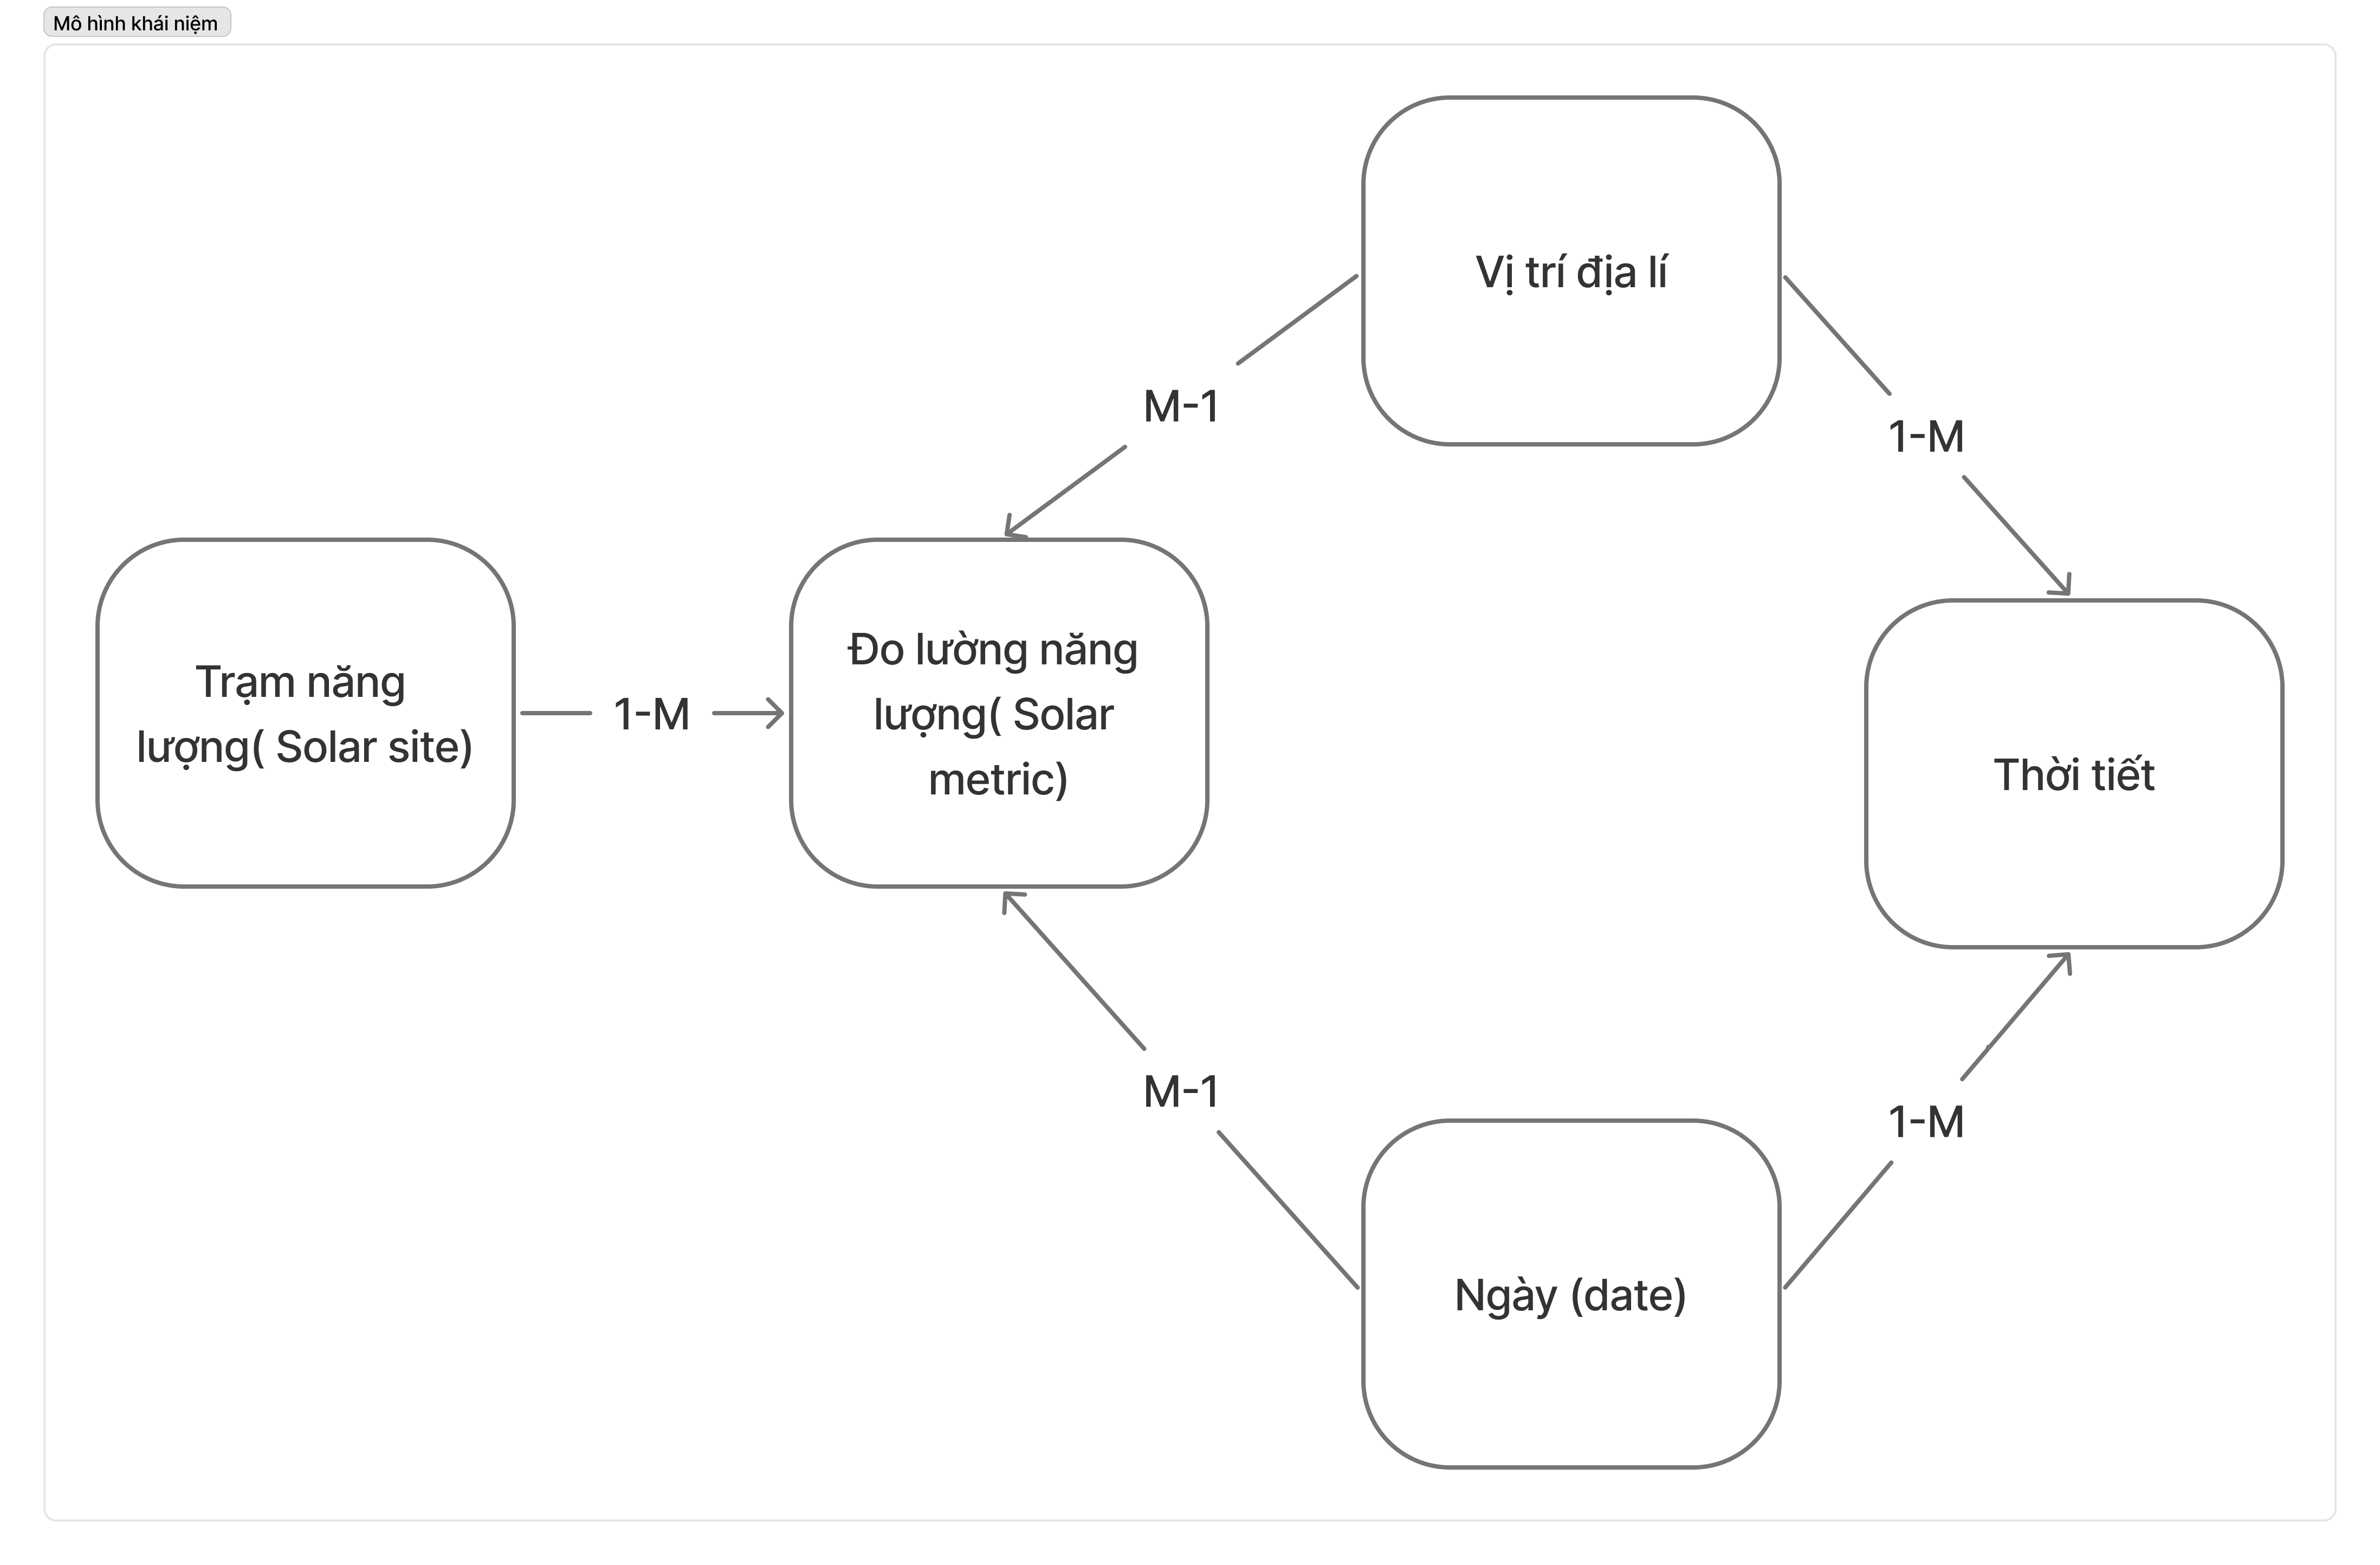
\includegraphics[width=0.88\textwidth]{figures/conceptual_model.png}
\caption{Sơ đồ mô hình khái niệm (Conceptual Model) thể hiện mối quan hệ giữa các thực thể hệ thống điện mặt trời.}
\label{fig:conceptual_model}
\end{figure}

\begin{figure}[H]
\centering
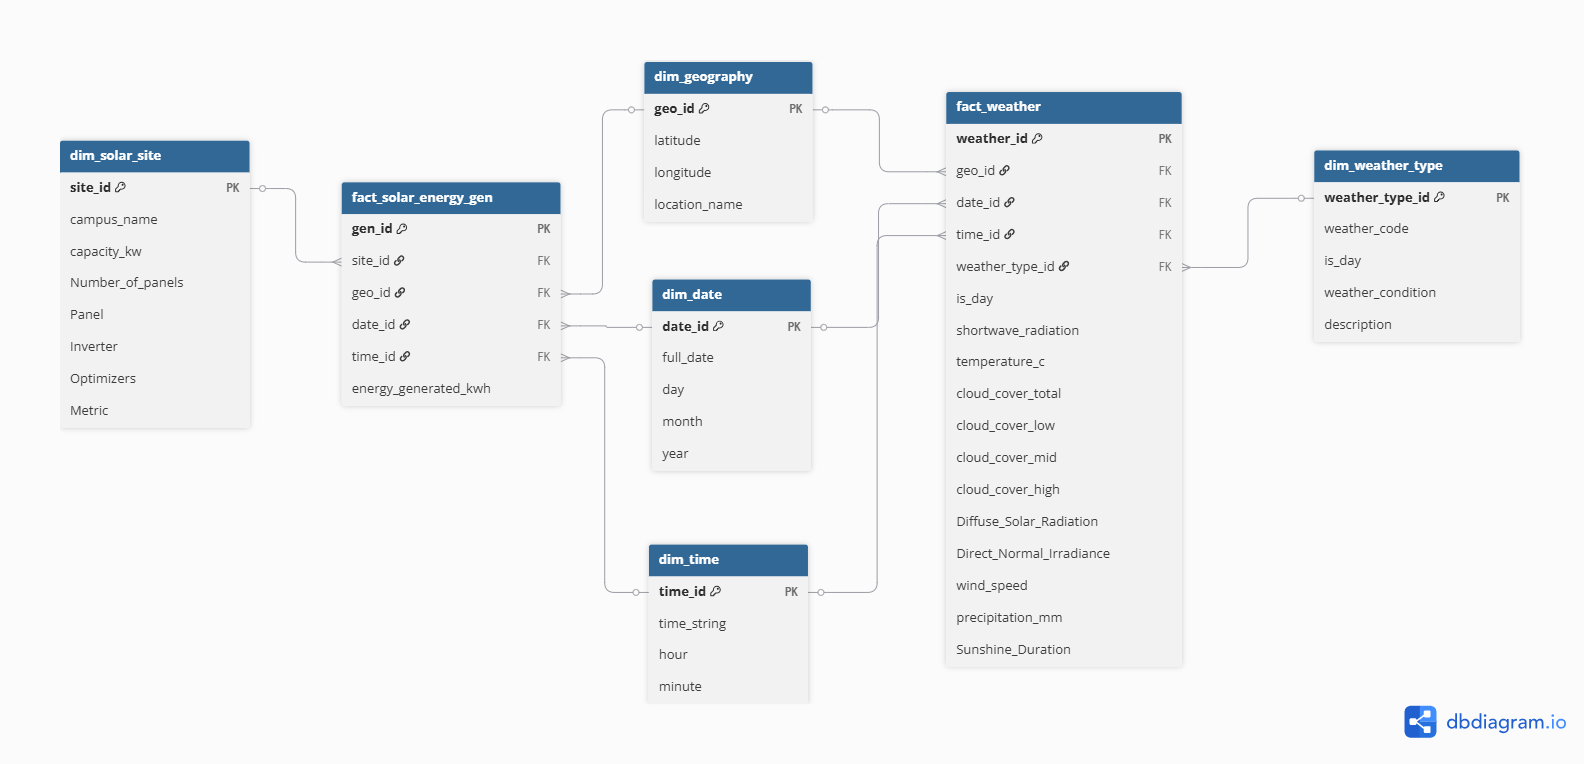
\includegraphics[width=0.92\textwidth]{figures/logical_model.png}
\caption{Sơ đồ mô hình logic (Logical Model) theo kiến trúc Galaxy Schema kết nối 2 bảng Fact và 4 bảng Dimension dùng chung.}
\label{fig:logical_model}
\end{figure}

\begin{figure}[H]
\centering
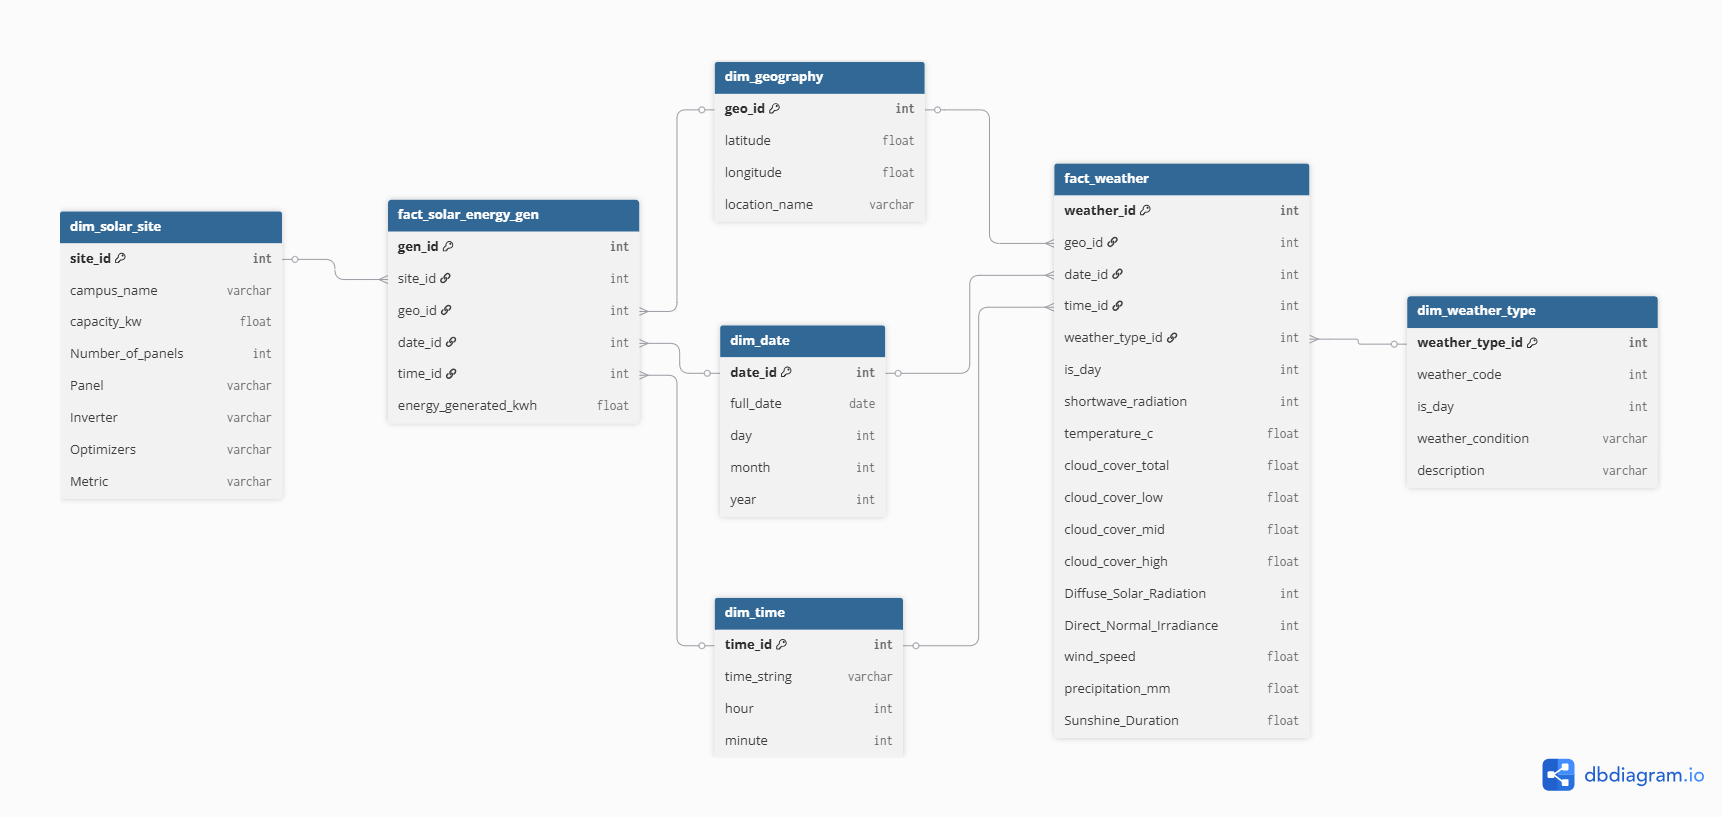
\includegraphics[width=0.95\textwidth]{figures/physical_model.png}
\caption{Sơ đồ mô hình vật lý (Physical Model) triển khai thực tế trên PostgreSQL Supabase.}
\label{fig:physical_model}
\end{figure}

\subsection{Cấu trúc Các Bảng trong Kho Dữ liệu}
\begin{enumerate}[noitemsep]
    \item \textbf{\texttt{dim\_solar\_plant} (Bảng Chiều Trạm phát):} 42 trạm phát với thông tin công suất danh định (\texttt{capacity\_kw}), khuôn viên (\texttt{campus\_name}) và vị trí địa lý.
    \item \textbf{\texttt{dim\_date} (Bảng Chiều Ngày):} 851 ngày lịch biểu trong chu kỳ 28 tháng với các thuộc tính phân tích thời gian.
    \item \textbf{\texttt{dim\_time} (Bảng Chiều Giờ):} 96 mốc thời gian vi mô 15 phút trong ngày.
    \item \textbf{\texttt{dim\_weather\_type} (Bảng Chiều Thời tiết):} Danh mục mã thời tiết chuẩn WMO.
    \item \textbf{\texttt{fact\_solar\_energy\_gen} (Bảng Sự kiện Sản lượng):} $2.731.946$ bản ghi sản lượng 15 phút kèm cờ dị thường và mã lý do.
    \item \textbf{\texttt{fact\_weather} (Bảng Sự kiện Khí tượng):} Các thông số bức xạ và thời tiết chu kỳ 1 giờ.
\end{enumerate}

\section{Tạo Bảng Tổng hợp và Siêu thị Dữ liệu (Siêu thị dữ liệu chuyên đề)}
\label{sec:data_marts}

Để đảm bảo các Dashboard trên Tableau tải tức thời (dưới 1 giây) khi các nhà quản lý thực hiện lọc dữ liệu, module \texttt{aggregate.py} thực hiện tính toán trước (Pre-calculated Aggregation) các bảng Data Marts chuyên biệt:

\begin{itemize}[noitemsep]
    \item \textbf{\texttt{agg\_daily\_plant\_performance.csv}:} Tổng hợp sản lượng hàng ngày, chỉ số PR trung bình, Specific Yield và tổn thất ước tính của 42 trạm phát.
    \item \textbf{\texttt{agg\_monthly\_campus\_summary.csv}:} Tổng hợp sản lượng theo tháng của 4 khuôn viên trường phục vụ báo cáo xu hướng tăng trưởng YoY.
    \item \textbf{\texttt{agg\_hourly\_temperature\_efficiency.csv}:} Ma trận tương quan giữa các dải nhiệt độ, bức xạ và hiệu suất chuyển đổi, làm nổi bật điểm suy giảm hiệu suất do nhiệt độ.
    \item \textbf{\texttt{agg\_anomaly\_diagnostic\_summary.csv}:} Thống kê số lượng và tỷ lệ của 6 mã lý do dị thường theo từng trạm phát phục vụ phân tích bảo trì O\&M.
\end{itemize}

\section{Kiểm tra Tính Toàn vẹn và Bảo mật Dữ liệu}
\label{sec:integrity_security}

\begin{enumerate}[noitemsep]
    \item \textbf{Kiểm tra Khóa ngoại (Anti-Join Check):} Thực hiện truy vấn Anti-Join giữa bảng Fact và Dimension, đảm bảo $100\%$ bản ghi có khóa tham chiếu hợp lệ (0 bản ghi mồ côi).
    \item \textbf{Xác thực Toàn vẹn Dữ liệu (Fingerprint Checksum MD5):} Hàm \texttt{fingerprint\_supabase()} đối chiếu mã băm MD5, tổng sản lượng ($74.982.150{,}45\,\text{kWh}$) và tổng số $2.731.946$ dòng dữ liệu trước và sau quá trình nạp để ngăn ngừa mất mát dữ liệu.
    \item \textbf{Bảo mật Phân quyền (Row-Level Security -- RLS):} Phân quyền truy cập an toàn trên Supabase Cloud, cấp quyền chỉ đọc (Read-only) cho Dashboard Tableau và tài khoản quản trị cho kỹ sư dữ liệu.
\end{enumerate}


% ====================================================================
%  CHƯƠNG 4: QUY TRÌNH ETL VÀ CHUẨN HÓA DỮ LIỆU
% ====================================================================
\chapter{Phát hiện Dị thường và Làm sạch Dữ liệu Nâng cao}
\label{chap:etl_cleaning}

\section{Tổng quan Kiến trúc Pipeline Xử lý Dữ liệu}
\label{sec:pipeline_overview}

Để xây dựng một hệ thống phân tích dữ liệu sản lượng điện mặt trời ổn định và tin cậy, dự án thiết lập quy trình trích xuất, biến đổi và nạp dữ liệu (ETL Pipeline) tự động hóa bằng ngôn ngữ Python. Luồng di chuyển dữ liệu (Data Flow) được chia làm 3 tầng lõi rõ rệt nhằm đáp ứng triết lý thiết kế kho dữ liệu tập trung (Top-Down Approach):

\begin{enumerate}[noitemsep]
    \item \textbf{Tầng Trích xuất (Extract):} Dữ liệu lịch sử từ các tệp tin CSV vật lý ghi nhận tại trạm pin và dữ liệu khí tượng viễn thám từ Open-Meteo API được thu thập và lưu trữ tập trung tại thùng chứa (Bucket) \texttt{raw-data} của hệ thống lưu trữ đối tượng MinIO S3. Các tệp tin cốt lõi bao gồm \texttt{campus\_meta.csv}, \texttt{Solar\_Site\_Details.csv}, \texttt{calender.csv}, \texttt{Solar\_Energy\_Generation.csv}, và \texttt{open\_meteo\_weather\_raw\_2020\_2022.csv}.
    \item \textbf{Tầng Biến đổi (Transform):} Sử dụng các thư viện tính toán hiệu năng cao như \texttt{pandas}, \texttt{numpy}, và \texttt{scikit-learn} để thực hiện chuẩn hóa kiểu dữ liệu thời gian, điền khuyết thiếu bằng chiến lược lai (Hybrid Imputation), gán cờ ngoại lai thông qua phân tích biến động trung bình trượt cục bộ, và đồng bộ granularity thời gian.
    \item \textbf{Tầng Nạp (Load):} Dữ liệu sau biến đổi được đẩy vào hệ quản trị cơ sở dữ liệu Supabase PostgreSQL thông qua hai schema chuyên biệt: \texttt{staging} (bộ đệm trung gian) và \texttt{datawarehouse} (kho dữ liệu chuẩn hóa đa chiều phục vụ BI và ML).
\end{enumerate}

Để khắc phục các hạn chế về môi trường triển khai thực tế, mã nguồn ETL của dự án tích hợp hai giải pháp hệ thống quan trọng:
\begin{itemize}
    \item \textbf{Sử dụng Thư viện kết nối thuần Python (\texttt{pg8000}):} Khác với thư viện \texttt{psycopg2} vốn yêu cầu biên dịch các thư viện hệ thống nhị phân C (dễ gây lỗi thiếu \texttt{libz.so.1} hoặc \texttt{libstdc++.so.6} trên môi trường ảo hóa NixOS), thư viện \texttt{pg8000} hoạt động hoàn toàn độc lập, đảm bảo tính di động cao của mã nguồn.
    \item \textbf{Cấu hình Connection Pooler thông qua IPv4:} Do Supabase chỉ hỗ trợ truy cập IPv6 trực tiếp cho gói tài khoản miễn phí, dự án cấu hình Pooler trung gian của Supabase tại cổng \texttt{5432} để duy trì kết nối IPv4 ổn định cho toàn bộ thành viên nhóm, đồng thời giảm tải luồng kết nối đồng thời lên máy chủ.
\end{itemize}

Dưới đây là mã nguồn cấu hình kết nối tối ưu hóa bằng thư viện \texttt{pg8000}:

\begin{lstlisting}[language=Python, caption={Mã nguồn thiết lập kết nối cơ sở dữ liệu qua Pooler bằng pg8000}, label={lst:pg8000_conn}]
def connect_pg8000() -> any:
    import pg8000.dbapi
    load_dotenv(ENV_FILE)
    required = ["DB_HOST", "DB_PORT", "DB_NAME", "DB_USER", "DB_PASSWORD"]
    missing = [name for name in required if not os.getenv(name)]
    if missing:
        raise RuntimeError(f"Missing env vars in {ENV_FILE}: {', '.join(missing)}")

    return pg8000.dbapi.connect(
        host=os.environ["DB_HOST"],
        port=int(os.environ.get("DB_PORT", "5432")),
        database=os.environ["DB_NAME"],
        user=os.environ["DB_USER"],
        password=os.environ["DB_PASSWORD"],
        ssl_context=True,
    )
\end{lstlisting}

\subsection{Thiết lập Tiến trình Nạp Dữ liệu Thứ tự}
Để bảo toàn tính toàn vẹn tham chiếu khóa ngoại (Foreign Key Constraints), tiến trình tải dữ liệu vào kho được kiểm soát nghiêm ngặt theo thứ tự phụ thuộc. File \texttt{load\_01\_dims.py} chịu trách nhiệm tẩy trống dữ liệu cũ bằng lệnh \texttt{TRUNCATE CASCADE} và tải lại các bảng chiều độc lập theo trình tự tuyến tính:
\begin{equation*}
\text{dim\_geography} \longrightarrow \text{dim\_solar\_site} \longrightarrow \text{dim\_date} \longrightarrow \text{dim\_time} \longrightarrow \text{dim\_weather\_type}
\end{equation*}

Ngay sau khi các bảng chiều được nạp thành công, tệp tin \texttt{load\_02\_facts.py} tiến hành đọc các bảng sự kiện quy mô lớn từ MinIO và ánh xạ các khóa tự nhiên sang khóa đại diện (Surrogate Keys) bằng các bộ từ điển tra cứu (Lookups) đã lưu trong bộ nhớ tạm (In-memory dicts). Để tránh hiện tượng nghẽn bộ nhớ đệm (RAM Out-Of-Memory) khi xử lý tập dữ liệu sản lượng hơn 2,7 triệu dòng, luồng nạp sử dụng cơ chế chia nhỏ dữ liệu thành từng khối (chunksize = 50.000 dòng) và thực thi lệnh chèn hàng loạt \texttt{execute\_values} tối ưu hóa hiệu năng IO.

\subsection{Cơ chế Quản lý Giao dịch và An toàn Dữ liệu}
Toàn bộ tiến trình nạp được bọc trong một khối giao dịch cơ sở dữ liệu duy nhất (Explicit DB Transaction). Chế độ tự động xác nhận (\texttt{autocommit}) được tắt hoàn toàn. 
\begin{itemize}
    \item Nếu xuất hiện bất kỳ lỗi hệ thống hoặc vi phạm ràng buộc dữ liệu nào (ví dụ: khóa ngoại không tồn tại), lệnh \texttt{conn.rollback()} sẽ lập tức hoàn tác mọi thay đổi để đưa kho dữ liệu về trạng thái an toàn trước đó.
    \item Chỉ khi toàn bộ dữ liệu của phân đoạn được ghi thành công không lỗi, lệnh \texttt{conn.commit()} mới được phát ra để ghi nhận vĩnh viễn các thay đổi vào đĩa cứng.
\end{itemize}

\section{Đánh giá Chất lượng và Khám phá Dữ liệu (EDA ban đầu)}
\label{sec:data_quality}

Trước khi thực hiện các phép toán làm sạch, nhóm tiến hành một bước hồ sơ hóa dữ liệu (Data Profiling) nhằm phát hiện các vấn đề về chất lượng dữ liệu thô. Tiến trình này được tự động hóa thông qua kịch bản \texttt{data\_integrity\_and\_reconciliation\_check.py}. 

Công cụ thực hiện quét toàn bộ các bảng trong schema \texttt{staging} để thống kê: (1) Tổng số dòng dữ liệu hiện có, (2) Số lượng bản ghi bị khuyết thiếu khóa chính (NULL PK), và (3) Số lượng bản ghi bị trùng lặp khóa tự nhiên (Duplicate PKs). 

\begin{table}[H]
\centering
\caption{Bảng thống kê kiểm tra chất lượng dữ liệu ban đầu trong Staging}
\label{tab:data_quality_report}
\renewcommand{\arraystretch}{1.3}
% Sử dụng >{\centering\arraybackslash}X để biến các cột số liệu thành cột tự động căn giữa và tự động xuống dòng
\begin{tabularx}{\textwidth}{l >{\centering\arraybackslash}X >{\centering\arraybackslash}X >{\centering\arraybackslash}X}
\toprule
\textbf{Tên bảng dữ liệu} & \textbf{Tổng số dòng} & \textbf{Số dòng trùng lặp} & \textbf{Số dòng khuyết PK} \\
\midrule
\texttt{dim\_geography}    & 5          & 0                  & 0                 \\
\texttt{dim\_solar\_site}  & 42         & 0                  & 0                 \\
\texttt{dim\_date}         & 2.312       & 0                  & 0                 \\
\texttt{dim\_time}         & 96         & 0                  & 0                 \\
\texttt{dim\_weather\_type}& 22         & 0                  & 0                 \\
\texttt{fact\_weather}     & 367.920     & 0                  & 0                 \\
\texttt{fact\_solar\_energy\_gen} & 2.731.946 & 0            & 0                 \\
\bottomrule
\end{tabularx}
\end{table}

Kết quả phân tích ban đầu cho thấy cấu trúc khung của các bảng chiều và bảng thời tiết rất sạch, không xuất hiện hiện tượng trùng lặp dòng. Tuy nhiên, bảng sự kiện sản lượng thô \texttt{fact\_solar\_energy\_gen} chứa tới 107.452 ô dữ liệu bị khuyết giá trị sản lượng (\texttt{SolarGeneration} mang giá trị \texttt{NaN}), chiếm khoảng 3,93\% tổng số quan trắc đo đạc của cả năm. Đây là đối tượng trọng tâm cần xử lý tại tầng làm sạch dữ liệu.

\subsection{Các Cột Thực Tế và Ánh Xạ Dữ Liệu Trong Pipeline}
Trong giai đoạn nạp dữ liệu từ các tệp thô vào bảng đệm (Staging layer), hệ thống thực hiện chuyển đổi kiểu dữ liệu (casting) và đổi tên trường để phù hợp với định dạng kho dữ liệu. Chi tiết các trường thông tin thực tế được ánh xạ từ tệp thô lên bảng sự kiện được thể hiện qua mã nguồn xử lý trực tiếp dưới đây:

\subsubsection{Cấu trúc ánh xạ bảng sự kiện sản lượng (\texttt{fact\_solar\_energy\_gen})}
Bảng này ghi nhận sản lượng điện thực tế theo chu kỳ 15 phút của từng trạm phát:
\begin{itemize}
    \item \texttt{sitekey} (Ánh xạ từ cột \texttt{SiteKey} trong tệp thô, định dạng chuỗi chuyển sang \texttt{VARCHAR} hoặc \texttt{INT}): Mã định danh duy nhất của từng trạm phát.
    \item \texttt{timestamp} (Ánh xạ từ cột \texttt{Timestamp} dạng text thô, xử lý chuyển đổi định dạng \texttt{YYYY-MM-DD HH24:MI:SS} sang kiểu dữ liệu \texttt{TIMESTAMP} chuẩn): Mốc thời gian quan trắc sản lượng.
    \item \texttt{energy\_generated\_kwh} (Ánh xạ từ cột \texttt{SolarGeneration} thô, làm sạch ký tự lạ và chuyển đổi thành \texttt{DOUBLE PRECISION} hoặc \texttt{FLOAT}): Sản lượng điện mặt trời thực tế thu được trong 15 phút (đơn vị kWh).
\end{itemize}

\subsubsection{Cấu trúc ánh xạ bảng sự kiện thời tiết (\texttt{fact\_weather})}
Thay vì chỉ liệt kê thủ công, toàn bộ logic trích xuất, ép kiểu dữ liệu từ nguồn khí tượng thô \texttt{staging.stg\_open\_meteo\_weather\_raw} (lấy từ Open-Meteo API~\cite{openmeteo2023}) sang bảng sự kiện \texttt{fact\_weather} được hiện thực hóa qua định nghĩa \texttt{LoadSpec} trong tệp tin mã nguồn \texttt{srcs/02\_transform/01\_run\_transform\_buffers.py}:

\begin{lstlisting}[language=Python, caption={Mã nguồn Python/SQL thực tế ánh xạ và chuyển đổi kiểu dữ liệu cho bảng sự kiện fact\_weather}, label={lst:fact_weather_mapping}]
LoadSpec(
    table="fact_weather",
    columns=(
        "sitekey",
        "timestamp",
        "weather_code",
        "is_day",
        "shortwave_radiation",
        "temperature_c",
        "cloud_cover_total",
        "cloud_cover_low",
        "cloud_cover_mid",
        "cloud_cover_high",
        "diffuse_solar_radiation",
        "direct_normal_irradiance",
        "wind_speed",
        "precipitation_mm",
        "sunshine_duration",
    ),
    select_sql=\"\"\"
        SELECT
            sitekey,
            timestamp::timestamp AS timestamp,
            weather_code::int AS weather_code,
            is_day::int AS is_day,
            shortwave_radiation::numeric 
                AS shortwave_radiation,
            temperature_2m::numeric 
                AS temperature_c,
            cloud_cover::numeric 
                AS cloud_cover_total,
            cloud_cover_low::numeric 
                AS cloud_cover_low,
            cloud_cover_mid::numeric 
                AS cloud_cover_mid,
            cloud_cover_high::numeric 
                AS cloud_cover_high,
            diffuse_radiation::numeric 
                AS diffuse_solar_radiation,
            direct_radiation::numeric 
                AS direct_normal_irradiance,
            wind_speed_10m::numeric 
                AS wind_speed,
            precipitation::numeric 
                AS precipitation_mm,
            sunshine_duration::numeric 
                AS sunshine_duration
        FROM staging.stg_open_meteo_weather_raw
    \"\"\",
)
\end{lstlisting}

Đoạn mã trên thể hiện rõ quy tắc chuẩn hóa kiểu dữ liệu nghiêm ngặt: mốc thời gian được ép về \texttt{TIMESTAMP}, mã thời tiết \texttt{weather\_code} và cờ \texttt{is\_day} ép về \texttt{INT}, trong khi tất cả 11 biến khí tượng viễn thám liên tục (bức xạ mặt trời, nhiệt độ 2m, các tầng mây che phủ, tốc độ gió 10m, lượng mưa và thời lượng nắng) đều được ép kiểu \texttt{NUMERIC} để bảo toàn độ chính xác số học cao nhất cho các phép tính tổn thất và mô hình học máy.

\section{Làm sạch và Chuẩn hóa Dữ liệu (Data Cleaning)}
\label{sec:cleaning}

\subsection{Xử lý Dữ liệu Khuyết thiếu và Lỗi Logic}
\label{subsec:null_imputation}

Để phục hồi dữ liệu khuyết thiếu cho trường sản lượng phát điện (\texttt{energy\_generated\_kwh}), dự án áp dụng chiến lược nội suy lai nghiêm ngặt (Hybrid Imputation Strategy) tích hợp giữa các bộ quy tắc nghiệp vụ vật lý và mô hình học máy trong file \texttt{solar\_data\_pipeline.py}. Tiến trình xử lý gồm hai giai đoạn chính:

\subsubsection{Giai đoạn 1: Lọc vật lý ban đêm (Rule-Based Night Zeroing)}
Đối với các trạm phát điện mặt trời quang điện, sản lượng điện năng luôn bằng 0 vào ban đêm do không có bức xạ mặt trời. Nếu sử dụng các thuật toán nội suy thuần toán học (như tuyến tính hay spline) trên các khoảng trống kéo dài qua đêm, hệ thống sẽ sinh ra các giá trị sản lượng ảo (dương) phi vật lý. 

Do đó, thuật toán tiến hành rà soát mốc thời gian và áp đặt giá trị 0 ngay lập tức nếu thỏa mãn một trong hai điều kiện logic sau:
\begin{itemize}
    \item \textbf{Khung giờ ban đêm tự nhiên:} Mốc thời gian đo đạc nằm trong khoảng từ 18:30 chiều hôm trước đến 05:30 sáng hôm sau ($T \ge 18.5$ hoặc $T < 5.5$).
    \item \textbf{Điều kiện thời tiết triệt tiêu:} Giá trị bức xạ sóng ngắn mặt trời (\texttt{shortwave\_radiation}) bằng 0 hoặc cờ chỉ số ánh sáng ngày \texttt{is\_day} bằng 0 trong tập dữ liệu thời tiết (được đồng bộ hóa sang dòng sản lượng tương ứng bằng thuật toán ghép nối mốc gần nhất \texttt{pd.merge\_asof} với ngưỡng sai lệch thời gian tối đa là 30 phút).
\end{itemize}
Giai đoạn này đã xử lý thành công 94.618 ô dữ liệu trống (chiếm tới 88,1\% tổng số giá trị khuyết thiếu ban đầu), gán chúng về giá trị \texttt{0.0} một cách chính xác.

Mã nguồn Python hiện thực thuật toán lọc vật lý ban đêm:

\begin{lstlisting}[language=Python, caption={Mã nguồn Python hiện thực bộ quy tắc Night-Zeroing vật lý}, label={lst:night_zero}]
def rule_based_night_zero(
    solar_df: pd.DataFrame, weather_df: pd.DataFrame, site_key: int
) -> tuple:
    gen = solar_df["energy_generated_kwh"].copy()
    ts = solar_df["timestamp"]

    # Xac dinh gio dem tu nhien
    hour = ts.dt.hour + ts.dt.minute / 60
    is_night = (hour >= NIGHT_START + 0.5) | (hour < NIGHT_END + 0.5)

    # Ket noi voi open_meteo de lay thong tin buc xa song ngan
    w = weather_df[weather_df["sitekey"] == site_key][
        ["timestamp", "shortwave_radiation", "is_day"]
    ].copy()
    w = w.rename(columns={"timestamp": "timestamp"})
    w["timestamp"] = pd.to_datetime(w["timestamp"])

    merged = pd.merge_asof(
        solar_df[["timestamp"]].reset_index(),
        w.sort_values("timestamp"),
        on="timestamp",
        tolerance=pd.Timedelta("30min"),
        direction="nearest",
    ).set_index("index")

    # Dieu kien buc xa song ngan bang 0 hoac co dem is_day = 0
    zero_radiation = (merged["shortwave_radiation"].fillna(0) == 0) | (
        merged["is_day"].fillna(0) == 0
    )
    mask_zero = is_night.values | zero_radiation.values

    n_filled = (mask_zero & gen.isna()).sum()
    gen[mask_zero & gen.isna()] = 0.0
    return gen, n_filled
\end{lstlisting}

\subsubsection{Giai đoạn 2: Nội suy phân cấp theo quy mô khoảng trống (Imputation Gaps classification)}
Đối với 12.834 ô dữ liệu khuyết thiếu phát sinh vào ban ngày (khi có bức xạ), thuật toán tiến hành phân tích độ dài chuỗi khuyết liên tiếp (Gap size) của từng trạm phát độc lập để áp dụng phương pháp điền khuyết tối ưu:

\begin{enumerate}[label=\alph*., leftmargin=*]
    \item \textbf{Khoảng khuyết ngắn ($\le 2$ dòng liên tiếp, tương đương $\le 30$ phút):} Áp dụng phương pháp nội suy tuyến tính (\textit{Linear Interpolation}) theo thời gian. Do khoảng thời gian gián đoạn rất ngắn, biến động của ánh sáng mặt trời được coi là thay đổi tuyến tính đều giữa điểm biên trước và biên sau khoảng khuyết.
    \item \textbf{Khoảng khuyết trung bình (Từ 3 đến 8 dòng liên tiếp, tương đương từ 45 phút đến 2 tiếng):} Áp dụng phương pháp nội suy \textit{Cubic Spline}. Đường cong bậc ba giúp mô phỏng mượt mà sự trồi sụt tự nhiên của sản lượng điện do mây che phủ đi qua trạm pin. Để tránh hiện tượng sập nhiễu ma trận khi gặp các khoảng khuyết lớn lân cận, thuật toán xây dựng một bản sao tạm thời được điền tuyến tính để làm mịn dữ liệu mốc trước khi tính toán spline bậc ba thực tế.
    \item \textbf{Khoảng khuyết diện rộng ($> 8$ dòng liên tiếp, tương đương $> 2$ tiếng):} Trong trường hợp này, dữ liệu bị mất quá dài khiến các phương pháp nội suy chuỗi đơn biến (Tuyến tính/Spline) mất khả năng phục hồi chính xác xu hướng thực tế. Nhóm thiết lập mô hình hồi quy đa biến (\textit{Multivariate Regression Imputation}) độc lập cho từng trạm phát.
    
    Mô hình Hồi quy Tuyến tính (\texttt{LinearRegression} từ thư viện \texttt{scikit-learn}) được huấn luyện trên tập các bản ghi sạch (đầy đủ thông tin) của chính trạm đó. Các biến đầu vào (Features) bao gồm: bức xạ sóng ngắn mặt trời (\texttt{shortwave\_radiation}), bức xạ chiếu trực tiếp (\texttt{direct\_normal\_irradiance}), bức xạ khuếch tán (\texttt{diffuse\_solar\_radiation}) và nhiệt độ không khí ở độ cao 2m (\texttt{temperature\_c}). 
    
    Sau khi huấn luyện, mô hình sẽ dự đoán sản lượng điện năng cho các khoảng khuyết diện rộng dựa trên dữ liệu khí tượng thực tế tại tọa độ trạm phát đó. Kết quả dự đoán được cắt giới hạn dưới bằng 0 (\texttt{clip(lower=0)}) để loại bỏ các giá trị âm sinh ra do sai số hồi quy.
\end{enumerate}

Mã nguồn Python thực thi hồi quy đa biến điền khuyết diện rộng ban ngày:

\begin{lstlisting}[language=Python, caption={Mã nguồn Python thực thi Multivariate Regression Imputation cho các khoảng khuyết lớn}, label={lst:regression_impute}]
def regression_imputation_large_gaps_strict(
    solar_sub: pd.DataFrame,
    weather_df: pd.DataFrame,
    site_key: int,
    large_gap_indices: set,
) -> tuple:
    FEATURES = [
        "shortwave_radiation",
        "direct_normal_irradiance",
        "diffuse_solar_radiation",
        "temperature_c",
    ]

    w = weather_df[weather_df["sitekey"] == site_key][["timestamp"] + FEATURES].copy()
    w = w.rename(columns={"timestamp": "timestamp"})
    w["timestamp"] = pd.to_datetime(w["timestamp"])

    merged = pd.merge_asof(
        solar_sub[["timestamp", "energy_generated_kwh"]].reset_index(),
        w.sort_values("timestamp"),
        on="timestamp",
        tolerance=pd.Timedelta("60min"),
        direction="nearest",
    ).set_index("index")

    train_mask = merged["energy_generated_kwh"].notna() & merged[FEATURES].notna().all(
        axis=1
    )
    pred_mask = merged["energy_generated_kwh"].isna() & merged[FEATURES].notna().all(
        axis=1
    )

    filled = 0
    if train_mask.sum() < 10:
        return solar_sub["energy_generated_kwh"].values, 0

    X_train = merged.loc[train_mask, FEATURES].values
    y_train = merged.loc[train_mask, "energy_generated_kwh"].values

    # Chuan hoa thong so dac trung dau vao
    scaler = StandardScaler()
    X_train_sc = scaler.fit_transform(X_train)

    model = LinearRegression()
    model.fit(X_train_sc, y_train)

    if pred_mask.sum() > 0:
        X_pred = merged.loc[pred_mask, FEATURES].values
        X_pred_sc = scaler.transform(X_pred)
        y_pred = model.predict(X_pred_sc)

        result = solar_sub["energy_generated_kwh"].copy()
        pred_indices = merged[pred_mask].index.tolist()

        for pos, idx in enumerate(pred_indices):
            local_pos = solar_sub.index.get_loc(idx) if idx in solar_sub.index else None
            # Chi ghi vao cac vi tri thuoc khoang khuyet lon
            if local_pos is not None and local_pos in large_gap_indices:
                result.iloc[local_pos] = max(0.0, y_pred[pos])
                filled += 1

        return result.values, filled
    return solar_sub["energy_generated_kwh"].values, 0
\end{lstlisting}

Tổng hợp kết quả sau quy trình làm sạch dữ liệu khuyết thiếu:
\begin{itemize}
    \item Tổng số ô trống ban đầu: 107.452 ô (3,93\% dữ liệu).
    \item Số ô được điền qua lọc ban đêm (Night Zero): 94.618 ô.
    \item Số ô được điền qua nội suy tuyến tính (Linear): 3.652 ô.
    \item Số ô được điền qua nội suy đường cong (Cubic Spline): 5.124 ô.
    \item Số ô được điền qua mô hình học máy hồi quy (Regression): 4.058 ô.
    \item Số ô NULL còn lại trong kho dữ liệu: 0 ô (Điền khuyết thành công 100\%).
\end{itemize}

\subsection{Xử lý Dữ liệu Ngoại lai (Outliers) và Lọc nhiễu}
\label{subsec:outlier_processing}

Trong chuỗi thời gian vận hành thực tế của hệ thống điện mặt trời quang điện (PV), dữ liệu đo đạc từ các cảm biến dòng điện (CT) và đồng hồ đo năng lượng (Smart Meters) thường xuyên xuất hiện các điểm dị thường (Anomalies/Outliers). Nếu không được nhận diện và gắn cờ chính xác, các dữ liệu này sẽ làm biến dạng các chỉ số hiệu suất kỹ thuật (như PR, CF) và gây sai lệch nghiêm trọng cho mô hình huấn luyện học máy dự báo sản lượng.

\subsubsection{Bản chất Nghiệp vụ và Phân tích Nguyên nhân Phát sinh Ngoại lai}
Dựa trên các nghiên cứu kỹ thuật chuyên sâu về độ tin cậy quang điện áp mái từ Tổ chức Năng lượng Quốc tế (IEA-PVPS Task 13)~\cite{iea2023pvps} và khảo sát thực nghiệm tại 42 trạm PV của Đại học La Trobe (Úc)~\cite{wimalaratne2022unisolar}, các hiện tượng bất thường trong dữ liệu phát sinh từ 4 nhóm nguyên nhân vật lý cốt lõi:

\begin{enumerate}[label=\arabic*., leftmargin=*]
    \item \textbf{Sự cố Biến tần và Thiết bị Chuyển đổi (Inverter / Optimizer Failures):}
    Theo báo cáo của IEA-PVPS~\cite{iea2023pvps}, bộ biến tần (Inverter) là mắt xích có độ tin cậy thấp nhất trong toàn bộ vòng đời hệ thống PV. Thời gian trung bình giữa hai lần hỏng (MTBF) của Inverter ngắn hơn tấm pin quang điện từ 300 đến 500 lần. Lỗi Inverter chiếm tới \textbf{36\%} tổng sản lượng tổn thất do thiết bị vật lý gây ra, với tỷ lệ hư hỏng hàng năm dao động từ 1\% đến 15\%/năm. Khi Inverter bị ngắt mạch bảo vệ quá nhiệt (Thermal trip) hoặc hỏng linh kiện bán dẫn, sản lượng trạm sụt giảm đột ngột về 0 giữa ban ngày dù bức xạ mặt trời đang đạt đỉnh cực đại ($> 700 \, \text{W/m}^2$).

    \item \textbf{Hỏng Diode Bypass và Che bóng Cục bộ (Bypass Diode Faults \& Shading):}
    Khi một tấm pin trong chuỗi (String) bị che bóng bởi cây cối, bụi bẩn bám dính dày đặc (Soiling) hoặc hỏng diode bypass, dòng điện của toàn bộ chuỗi bị bóp nghẹt theo tấm pin yếu nhất. Sự cố diode bypass có thể làm triệt tiêu tới \textbf{33\%} sản lượng điện của riêng tấm pin đó, tạo nên các vết sụt giảm sản lượng cục bộ dạng bậc thang phi tự nhiên.

    \item \textbf{Suy giảm do Quá nhiệt và Điểm nóng (Thermal Derating \& Hot-spots):}
    Hệ số nhiệt độ (Temperature Coefficient) của pin silicon tinh thể dao động từ $-0{,}30\%$ đến $-0{,}50\%/^\circ\text{C}$ khi nhiệt độ vượt mốc điều kiện chuẩn STC ($25^\circ\text{C}$). Vào các ngày nắng gắt mùa hè, nhiệt độ bề mặt ô pin ($T_{\text{cell}}$) có thể tăng vọt lên tới $65^\circ\text{C}$, làm sụt giảm \textbf{12--20\%} công suất đỉnh chủ yếu do suy giảm điện áp hở mạch ($V_{oc}$). Nhiệt độ vượt ngưỡng $85--90^\circ\text{C}$ có thể gây ra hiện tượng điểm nóng (Hot-spots), dẫn đến suy thoái vĩnh viễn mối hàn và lớp phủ bảo vệ.

    \item \textbf{Nhiễu Cảm biến và Dòng điện Rò Ban đêm (Sensor Drift \& Night Leakage):}
    Hiện tượng rò rỉ dòng điện ngược (Reverse Current) từ lưới điện vào ban đêm hoặc cảm biến biến dòng (CT) bị trôi mốc 0 (Zero-drift fault) sinh ra các giá trị sản lượng dương giả mạo ($E > 0$) trong khoảng thời gian không có bức xạ ($18:30 - 05:30$). Ngoài ra, các xung nhiễu điện áp lưới (Voltage spikes) hoặc gián đoạn đường truyền viễn thông (Telemetry dropouts) tạo nên các đỉnh xung sản lượng vượt trần công suất thiết kế cực đại ($P > 1{,}2 \cdot P_{\text{stc}}$) hoặc các bước nhảy đột biến giữa các chu kỳ 15 phút kế cận.
\end{enumerate}

\subsubsection{Khung Thuật toán Phân lớp Lai GMM--IF và Rào chắn Vật lý}
Dữ liệu chuỗi thời gian quang điện có tính phi tuyến và phân phối đa đỉnh (Multimodal) biến động theo thời tiết, khiến các phương pháp thống kê toàn cục kinh điển (như $3\sigma$ hay Boxplot IQR truyền thống~\cite{tukey1977eda}) dễ nhận diện nhầm dữ liệu bình thường của ngày âm u thành ngoại lai. Nhằm khắc phục hạn chế này, nhóm mở rộng khung nghiên cứu của Li và cộng sự~\cite{li2025gmmif} trên tạp chí \textit{IEEE Access}, thiết lập mô hình lai phân lớp 3 tầng trong \texttt{srcs/02\_transform/02\_generate\_outliers/02\_gmm\_if.py}:

\begin{itemize}
    \item \textbf{Tầng 1 -- Phân đoạn Cây quyết định (Decision Tree Segmentation):} Sử dụng cây hồi quy quyết định để chia dữ liệu của từng trạm phát thành 19 đến 29 vùng vận hành lá (Leaf segments) dựa trên bức xạ sóng ngắn, nhiệt độ và mốc thời gian. Mỗi phân đoạn tạo thành một vùng dữ liệu cục bộ tương đối đồng nhất có phân phối xấp xỉ Gauss (hệ số $R^2$ trung bình đạt $0{,}758$).
    \item \textbf{Tầng 2 -- Ước lượng Mật độ Hỗn hợp Gauss (GMM)~\cite{bishop2006pattern}:} Trong từng phân đoạn lá, huấn luyện mô hình GMM 2 thành phần ($M = 2$) để đo lường mật độ xác suất $p(x)$. Các điểm dữ liệu nằm ở vùng mật độ cực thấp ($P_{\text{GMM}} < 0{,}02$) bị gắn nhãn ứng viên ngoại lai theo góc nhìn phân phối xác suất.
    \item \textbf{Tầng 3 -- Rừng cô lập (Isolation Forest -- IF)~\cite{liu2008isolation}:} Khởi tạo 100 cây ngẫu nhiên để đo lường số nhát cắt cần thiết nhằm cô lập điểm dữ liệu khỏi đám đông với tham số \texttt{contamination} $= 3\%$.
    \item \textbf{Cơ chế Hợp nhất Đồng thuận (Fusion Consensus $GMM \wedge IF$):} Một điểm dữ liệu chỉ được gắn cờ dị thường máy học khi \textbf{cả GMM và IF cùng đồng thuận}:
    \begin{equation}
        \text{Flag}_{\text{ML}} = \text{Flag}_{\text{GMM}} \wedge \text{Flag}_{\text{IF}}
    \end{equation}
    Phép giao logic này giúp triệt tiêu phần lớn các cảnh báo giả (False Positives) của từng mô hình riêng lẻ (chỉ số tương đồng Jaccard giữa hai thuật toán đạt từ $6{,}4\%$ đến $16{,}7\%$).
\end{itemize}

\begin{figure}[H]
\centering

\includegraphics[width=0.98\textwidth]{figures/gmm_if_architecture.png}
\caption{Sơ đồ kiến trúc mô hình phân lớp lai GMM--IF và rào chắn vật lý kết hợp quy trình 4 bước nạp cờ an toàn vào Supabase DWH.}
\label{fig:gmm_if_architecture}
\end{figure}

\subsubsection{Hệ thống Danh mục Mã Lý do Ngoại lai (\texttt{gmm\_if\_outlier\_reason})}
Để phục vụ cho hệ thống giám sát và bảo trì cảnh báo trên Dashboard Tableau, mỗi bản ghi bị gắn cờ được gán một mã nguyên nhân cụ thể thông qua hàm \texttt{explain\_outlier\_row()} trong \texttt{02\_gmm\_if.py}. Chi tiết 6 mã lý do kỹ thuật được chuẩn hóa tại Bảng~\ref{tab:outlier_reasons_dict}:

\begin{table}[H]
\centering
\small
\renewcommand{\arraystretch}{1.3}
\begin{tabularx}{\textwidth}{@{} l p{4.5cm} X @{}}
\toprule
\textbf{Mã Định danh Lý do} & \textbf{Định nghĩa Ngưỡng Kỹ thuật} & \textbf{Ý nghĩa Nghiệp vụ \& Chẩn đoán} \\
\midrule
\texttt{GMM\_IF\_CONSENSUS} & 
$\text{Flag}_{\text{GMM}} = \text{true}$ \textbf{và} $\text{Flag}_{\text{IF}} = \text{true}$ (Phép giao đồng thuận). & 
Bất thường đồng thời về mặt mật độ xác suất cục bộ và không gian phân tách toàn cục; cần kiểm tra cảm biến hoặc trạng thái vận hành trạm. \\
\midrule
\texttt{PHYSICAL\_OVER\_CAPACITY} & 
Sản lượng 15 phút vượt trần công suất lắp đặt: $E > \text{capacity\_kw} \times 0{,}25$. & 
Đỉnh phát điện vượt quá công suất định mức cực đại của dàn PV; cảnh báo xung điện lưới, lỗi telemetry hoặc sai lệch siêu dữ liệu trạm. \\
\midrule
\texttt{PHYSICAL\_HIGH\_ENERGY\_NO\_SUN} & 
$\text{shortwave\_radiation} \le 25 \, \text{W/m}^2$, $\text{sunshine} \le 60\text{s}$, nhưng $E \ge \max(1.0, 0{,}20 \cdot P_{\text{stc}})$. & 
Sản lượng điện cao trong điều kiện trời tối hoàn toàn; mâu thuẫn vật lý cảnh báo sự cố rò rỉ điện ban đêm (Night Leakage) hoặc dòng rò ngược. \\
\midrule
\texttt{PHYSICAL\_HIGH\_ENERGY\_LOW\_RAD} & 
$\text{shortwave\_radiation} \le 50 \, \text{W/m}^2$, $E \ge \max(1.0, 0{,}20 \cdot P_{\text{stc}})$, và $E > Q_3 + 4 \cdot \text{IQR}$. & 
Sản lượng cao bất thường khi bức xạ mặt trời rất yếu; vi phạm ngưỡng phân phối thống kê đuôi sâu của nhóm bức xạ tương ứng. \\
\midrule
\texttt{PHYSICAL\_LOW\_ENERGY\_STRONG\_SUN} & 
$\text{shortwave\_radiation} \ge 700 \, \text{W/m}^2$, $\text{sunshine} \ge 3000\text{s}$, $E \le 0{,}05 \cdot P_{95}$ và $E \le Q_1 - 2 \cdot \text{IQR}$. & 
Mất phát hoặc sụt giảm sản lượng nghiêm trọng trong điều kiện nắng cực đại; cảnh báo sự cố ngắt Inverter, hỏng diode bypass hoặc che bóng diện rộng. \\
\midrule
\texttt{PHYSICAL\_DISTRIBUTION\_JUMP} & 
Bỏ qua giờ chuyển tiếp (05h, 06h, 18h). $|E - E_{\text{neighbor}}| \ge \max(0{,}15 \cdot P_{95}, 1.0)$ và $E \notin [Q_1 - 4\text{IQR}, Q_3 + 4\text{IQR}]$. & 
Bước nhảy hoặc sụt giảm công suất cục bộ đột ngột so với diễn biến 2 giờ xung quanh; cảnh báo hiện tượng spike tín hiệu hoặc dropout truyền thông tin. \\
\bottomrule
\end{tabularx}
\caption{Danh mục các mã lý do ngoại lai được định nghĩa trong pipeline GMM--IF và ý nghĩa chẩn đoán bảo trì.}
\label{tab:outlier_reasons_dict}
\end{table}

Khi một bản ghi vi phạm đồng thời nhiều điều kiện, các mã lý do được nối với nhau bằng dấu cộng (Ví dụ: \texttt{GMM\_IF\_CONSENSUS+PHYSICAL\_DISTRIBUTION\_JUMP}), hỗ trợ kỹ sư vận hành phân rã đa tầng nguyên nhân sự cố.

\subsubsection{Quy trình Đẩy Cờ An toàn 4 Bước vào Kho Dữ liệu Supabase}
Để cập nhật cờ ngoại lai lên Supabase DWH mà không làm gián đoạn hệ thống và đảm bảo an toàn giao dịch tuyệt đối, nhóm xây dựng pipeline 4 bước trong mã nguồn \texttt{srcs/02\_transform/02\_run\_apply\_outlier\_flags.py}:
\begin{enumerate}
    \item \textbf{Xác thực nguồn dữ liệu (Source Verification Check):} Trước khi ghi dữ liệu, hàm \texttt{fingerprint\_supabase()} tiến hành đối chiếu cấu trúc vân tay dữ liệu giữa tệp kết quả phân tích ngoại lai và bảng sự kiện \texttt{fact\_solar\_energy\_gen} trên Supabase. 
    
    Quy trình kiểm tra tính toán tổng băm MD5 của chuỗi khóa ghép (\texttt{sitekey|timestamp}), tổng sản lượng năng lượng (\texttt{energy\_sum}) với sai số cho phép $\le 0{,}01$, và tổng số dòng dữ liệu. Bước này đảm bảo dữ liệu chạy cờ ngoại lai và dữ liệu trên cơ sở dữ liệu hoàn toàn đồng nhất về cấu trúc cột và số lượng dòng (2.731.946 dòng), ngăn ngừa lỗi lệch dòng (Data Shift).
    
    \item \textbf{Nạp danh sách ứng viên (Sparse Candidate Upload):} Thay vì tải lên lại toàn bộ 2,73 triệu dòng dữ liệu (rất chậm và dễ gây nghẽn mạng), thuật toán chỉ lọc ra 33.280 bản ghi bị gắn cờ ngoại lai thực sự (\texttt{gmm\_if\_outlier\_flag = true}). Danh sách ứng viên này được đẩy vào bảng tạm trung gian: \texttt{staging.temp\_gmm\_if\_outlier\_flags}.
    
    \item \textbf{Kiểm tra tính toàn vẹn khóa ngoại (Referential Check):} Thực hiện truy vấn kiểm tra chéo (Anti-Join) để đảm bảo toàn bộ các khóa trong bảng tạm đều tồn tại khớp 1:1 trong bảng sự kiện chính. Kết quả trả về 0 dòng lỗi trước khi tiến hành cập nhật.
    
    \item \textbf{Cập nhật giao dịch hàng loạt (Bulk Join Update):} Tiến trình mở một khối giao dịch an toàn trên cơ sở dữ liệu, thực hiện gán toàn bộ cờ \texttt{gmm\_if\_outlier\_flag = false} cho cả bảng sự kiện chính (2.731.946 dòng), sau đó thực hiện lệnh cập nhật \texttt{UPDATE ... FROM ... WHERE} nối bảng tạm với bảng chính theo khóa trùng khớp (\texttt{sitekey}, \texttt{timestamp}) để chuyển 33.280 dòng ngoại lai sang trạng thái \texttt{true} kèm mã lý do tương ứng.
\end{enumerate}

Dưới đây là một phần mã nguồn Python thực hiện so sánh đối chiếu vân tay (Fingerprint) dữ liệu trích từ \texttt{srcs/02\_transform/02\_run\_apply\_outlier\_flags.py}:

\begin{lstlisting}[language=Python, caption={Mã nguồn Python kiểm tra vân tay dữ liệu (Fingerprint) trước khi cập nhật}, label={lst:data_fingerprint}]
def fingerprint_supabase(conn: any) -> dict[str, object]:
    cur = conn.cursor()
    try:
        cur.execute(
            f"""
            SELECT
                COUNT(*)::bigint AS rows,
                COUNT(DISTINCT sitekey)::bigint AS sites,
                MIN(to_char(
                    timestamp, 'YYYY-MM-DD HH24:MI:SS'
                )),
                MAX(to_char(
                    timestamp, 'YYYY-MM-DD HH24:MI:SS'
                )),
                SUM(
                    energy_generated_kwh::numeric
                ) AS energy_sum,
                SUM(
                    ('x' || substr(
                        md5(sitekey::text || '|' || 
                        to_char(
                            timestamp, 
                            'YYYY-MM-DD HH24:MI:SS'
                        )),
                        1, 15
                    ))::bit(60)::bigint
                )::numeric AS key_checksum
            FROM {qname(SCHEMA, SOURCE_FACT_TABLE)}
            """
        )
        row = cur.fetchone()
        return {
            "rows": int(row[0]),
            "distinct_sitekeys": int(row[1]),
            "min_timestamp": row[2],
            "max_timestamp": row[3],
            "energy_sum": Decimal(str(row[4] or 0)),
            "key_checksum": Decimal(str(row[5] or 0)),
        }
    finally:
        cur.close()
\end{lstlisting}

\subsubsection{Kết quả Phân bổ và Đánh giá Kiểm toán Không Giám sát}
Vì đây là bài toán học máy không giám sát trên dữ liệu chuỗi thời gian thực tế không có nhãn sự cố thủ công từ người vận hành, hệ thống không thể sử dụng các chỉ số giả định như Accuracy, Precision hay Recall. Thay vào đó, chất lượng của bộ phát hiện ngoại lai được kiểm chứng thông qua bộ 4 chỉ số kiểm toán khoa học:

\begin{itemize}
    \item \textbf{Độ hội tụ mô hình GMM:} Đạt \textbf{100\%} trên toàn bộ 42 trạm phát (toàn bộ các phân đoạn lá cây quyết định đều hội tụ thuật toán EM thành công, không có segment nào bị lỗi fit).
    \item \textbf{Kiểm soát tỷ lệ nhiễu IF:} Isolation Forest giữ đúng tham số \texttt{contamination} xấp xỉ \textbf{3\%} trên từng trạm phát.
    \item \textbf{Chất lượng phân đoạn cây quyết định ($R^2$):} Hệ số $R^2$ đạt trung bình $\mathbf{0{,}758}$ (thấp nhất $0{,}606$, cao nhất $0{,}826$), chứng minh các vùng phân đoạn mô phỏng chính xác cấu trúc hình dạng phát điện của trạm.
    \item \textbf{Tổng số lượng bản ghi gắn cờ ngoại lai:} Toàn bộ pipeline đã gắn cờ thành công $\mathbf{33.280}$ dòng trên tổng số $\mathbf{2.731.946}$ dòng dữ liệu, tương ứng với tỷ lệ ngoại lai được kiểm soát ở mức lý tưởng $\mathbf{1{,}22\%}$.
\end{itemize}

\section{Biến đổi và Trích xuất Đặc trưng (Feature Engineering)}
\label{sec:transformation}

Sau khi dữ liệu sản lượng và thời tiết được làm sạch tại tầng kho dữ liệu, tiến trình thực hiện tính toán biến đổi cấu trúc để chuẩn bị dữ liệu đầu vào tối ưu cho mô hình dự báo học máy.

\subsection{Giải quyết độ lệch tần suất ghi nhận (Granularity Alignment)}
Một thách thức lớn trong dữ liệu của dự án là độ lệch tần suất (Granularity Mismatch) giữa hai nguồn thông tin nghiệp vụ:
\begin{itemize}
    \item Dữ liệu sản lượng điện được ghi nhận với tần suất cao (15 phút một dòng).
    \item Dữ liệu khí tượng viễn thám chỉ có sẵn theo chu kỳ giờ (60 phút một dòng).
\end{itemize}

Để giải quyết sự lệch pha này mà không làm mất mát thông tin xu hướng của bức xạ mặt trời, nhóm thiết lập thuật toán gom cụm (Aggregation) đưa dữ liệu về cùng chu kỳ giờ (1-hour grain). Chỉ số sản lượng điện mặt trời \texttt{energy\_generated\_kwh} trong 4 chu kỳ 15 phút của cùng một giờ được tính tổng cộng dồn (Sum Aggregation):
\begin{equation}
E_{\text{hour}} = \sum_{i=1}^{4} E_{15\text{min}, i}
\end{equation}
Trong khi đó, các biến thời tiết đại diện cho giờ đó được giữ nguyên giá trị trung bình giờ. Thuật toán ghép nối sử dụng hàm kết hợp chính xác mốc thời gian chẵn giờ, giúp tạo ra một bảng dữ liệu phẳng góc nhìn rộng (Wide-table) thống nhất, đảm bảo tính liên kết chặt chẽ và không có dữ liệu rò rỉ thời gian (Data Leakage).

\subsection{Trích xuất các đặc trưng thời gian và lịch trình học tập}
Điện năng mặt trời mang tính chu kỳ tự nhiên rất mạnh phụ thuộc vào quỹ đạo chuyển động của Trái Đất. Dự án tiến hành trích xuất các đặc trưng thời gian đa tầng từ trường mốc thời gian \texttt{timestamp}:
\begin{itemize}
    \item \textbf{Đặc trưng giờ trong ngày (Hour):} Giá trị từ 0 đến 23, xác định góc chiếu mặt trời.
    \item \textbf{Đặc trưng tháng trong năm (Month):} Xác định tính mùa vụ thời tiết (Mùa hè bức xạ cao, mùa đông bức xạ thấp ở Nam bán cầu).
    \item \textbf{Đặc trưng ngày trong tuần (Day of Week):} Hỗ trợ phân tích hành vi tiêu thụ điện năng tại các khu học xá (Campus).
\end{itemize}

Đặc biệt, nhóm tích hợp thành công dữ liệu lịch học tập (\texttt{calender.csv}) của cơ sở đào tạo thông qua ba đặc trưng nhị phân:
\begin{itemize}
    \item \texttt{is\_holiday}: Đánh dấu các ngày nghỉ lễ quốc gia hoặc ngày nghỉ nội bộ.
    \item \texttt{is\_semester}: Đánh dấu thời điểm đang trong học kỳ chính thức (nhu cầu sử dụng thiết bị điện cao đột biến).
    \item \texttt{is\_exam}: Đánh dấu giai đoạn thi cử tập trung.
\end{itemize}
Sự kết hợp các thuộc tính lịch trình này giúp mô hình học máy phân biệt rõ rệt giữa biến động sản lượng do thời tiết tự nhiên và biến động tiêu thụ do hành vi con người gây ra, cải thiện độ chính xác dự báo sản lượng thực dùng tại các điểm nút phụ tải trạm.


% ====================================================================
%  CHƯƠNG 5: TRỰC QUAN DỮ LIỆU VÀ XÂY DỰNG DASHBOARD
% ====================================================================
\chapter{Trực quan Dữ liệu và Xây dựng Dashboard}
\label{chap:dashboard}

\section{Chiến lược Kết nối Dữ liệu và Thiết kế UI/UX}
\label{sec:dashboard_strategy}

Trực quan hóa dữ liệu là cầu nối cốt lõi chuyển hóa các kết quả phân tích phức tạp từ hệ thống kho dữ liệu thành tri thức hành động (Actionable Insights) cho doanh nghiệp. Theo tinh thần chỉ đạo chuyên môn ``Không có câu hỏi $\rightarrow$ Không có phân tích'' và ``Đừng chỉ mô tả $\rightarrow$ Phải giải thích'', hệ thống Dashboard trên nền tảng Tableau được thiết kế theo tư duy tiếp cận từ trên xuống (Top-Down Approach), đáp ứng đa dạng nhu cầu của hai nhóm người dùng trọng yếu: Ban Giám đốc quản lý và Đội ngũ Kỹ sư Vận hành \& Bảo trì (O\&M).

\subsection{Quy trình Thiết lập Kết nối PostgreSQL Trực tiếp từ Supabase}
\label{subsec:db_connection}

Để khai thác dữ liệu trực tiếp từ Kho dữ liệu đám mây (Cloud Data Warehouse), hệ thống Tableau Desktop sử dụng trình kết nối gốc PostgreSQL (Native PostgreSQL Connector). Cơ chế này thiết lập đường truyền dữ liệu thời gian thực có mã hóa bảo mật TLS/SSL tới cơ sở dữ liệu Supabase lưu trữ trên hạ tầng AWS (khu vực Đông Nam Á \texttt{ap-southeast-1}).

\begin{figure}[H]
    \centering
    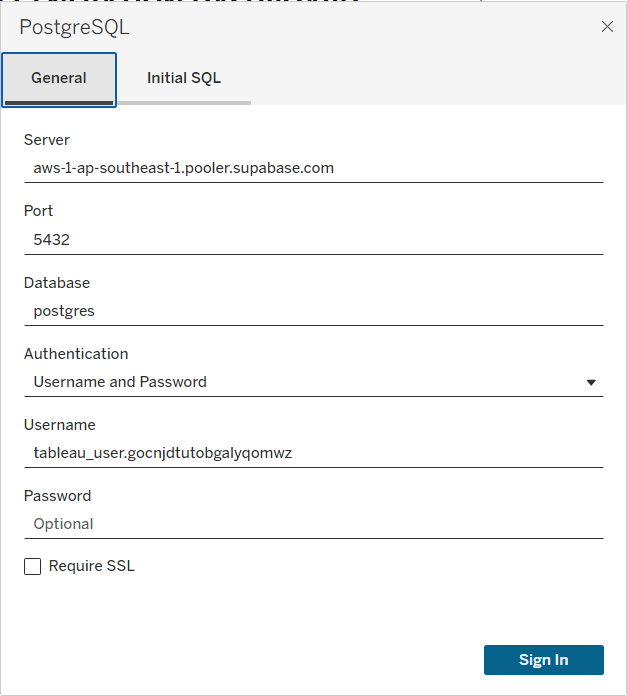
\includegraphics[width=0.62\textwidth]{figures/tableau_connect_supabase.png}
    \caption{Cửa sổ cấu hình kết nối PostgreSQL từ Tableau Desktop tới Supabase Data Warehouse}
    \label{fig:tableau_connect_supabase}
\end{figure}

Thông số cấu hình kết nối chi tiết giữa Tableau và hệ cơ sở dữ liệu PostgreSQL của dự án được chuẩn hóa như trong Bảng~\ref{tab:tableau_connection_params}:

\begin{table}[H]
\centering
\small
\renewcommand{\arraystretch}{1.25}
\begin{tabularx}{\textwidth}{@{} l l X @{}}
\toprule
\textbf{Tham số Kết nối} & \textbf{Giá trị Cấu hình} & \textbf{Ý nghĩa Kỹ thuật \& Bảo mật} \\
\midrule
\textbf{Connector Type} & PostgreSQL & Trình kết nối hiệu năng cao tối ưu hóa riêng cho PostgreSQL/Tableau. \\
\textbf{Server / Host} & \texttt{aws-1-ap-southeast-1.pooler.supabase.com} & Cổng Supabase Connection Pooler (AWS Singapore) giúp duy trì kết nối ổn định và tái sử dụng connection pool. \\
\textbf{Port} & \texttt{5432} & Cổng mạng tiêu chuẩn dành cho giao thức PostgreSQL Session Pool. \\
\textbf{Database} & \texttt{postgres} & Cơ sở dữ liệu đích chứa các schema \texttt{bi\_mart}, \texttt{gold}, \texttt{dim}. \\
\textbf{Authentication} & Username and Password & Xác thực danh tính người dùng bằng phương thức mã hóa định danh. \\
\textbf{Username} & \texttt{tableau\_user.gocnjdtutobgalyqomwz} & Tài khoản dịch vụ chuyên dụng (Dedicated Service Account) được phân quyền Read-only tối thiểu (Principle of Least Privilege) trên schema \texttt{bi\_mart}. \\
\textbf{Encryption} & Require SSL / TLS & Bắt buộc mã hóa toàn bộ luồng truyền tải dữ liệu giữa máy trạm BI và máy chủ Supabase. \\
\bottomrule
\end{tabularx}
\caption{Thông số thiết lập kết nối PostgreSQL từ Tableau tới Supabase Data Warehouse.}
\label{tab:tableau_connection_params}
\end{table}

Việc sử dụng cổng Pooler kết hợp tài khoản dịch vụ phân quyền độc lập mang lại 3 ưu điểm kỹ thuật vượt trội:
\begin{enumerate}[label=\arabic*., leftmargin=*]
    \item \textbf{Khả năng Chịu tải Cao (Concurrency Handling):} Cơ chế Connection Pooling tự động điều phối hàng trăm truy vấn phân tích song song từ các Dashboard mà không làm tràn bộ nhớ RAM của cụm máy chủ Supabase.
    \item \textbf{Bảo mật Dữ liệu Nghiêm ngặt (Least Privilege):} Tài khoản \texttt{tableau\_user} chỉ được cấp quyền \texttt{SELECT} trên tầng BI Mart và các bảng Dimension, ngăn chặn hoàn toàn rủi ro can thiệp thay đổi cấu trúc bảng hoặc ghi đè dữ liệu.
    \item \textbf{Độ trễ Truy vấn Cực thấp (Low Latency):} Cụm máy chủ đặt tại Datacenter Singapore (\texttt{ap-southeast-1}) đảm bảo thời gian phản hồi truy vấn dưới 1,5 giây cho mọi thao tác lọc tương tác từ Việt Nam.
\end{enumerate}

\subsection{Mô hình Kết nối Dữ liệu Tầng BI Mart và Tableau Relationships}
\label{subsec:bi_mart_model}

Để đảm bảo tốc độ phản hồi tính toán thời gian thực trên Tableau mà không gây quá tải cho hệ quản trị cơ sở dữ liệu Supabase PostgreSQL, dự án không thực hiện truy vấn trực tiếp trên các bảng sự kiện thô 2,7 triệu dòng. Thay vào đó, hệ thống Tableau kết nối trực tiếp với tầng BI Mart đã được tối ưu hóa sẵn thông qua hai Materialized Views lõi:
\begin{itemize}
    \item \texttt{bi\_mart.mv\_bi\_mart\_hourly\_measures}: Lưu trữ toàn bộ các đo lường chi tiết theo từng giờ của 42 trạm phát, bao gồm sản lượng thực tế (\texttt{e\_hourly}), sản lượng chuẩn STC (\texttt{e\_stc\_hourly}), sản lượng kỳ vọng hiệu chỉnh nhiệt (\texttt{e\_expected}), hệ số hiệu suất (\texttt{pr\_actual}, \texttt{pr\_adjusted}), suy hao do nhiệt (\texttt{loss\_temp}), nhiệt độ ô pin (\texttt{t\_cell}), cùng các cờ báo động ngoại lai GMM-IF (\texttt{gmm\_if\_outlier\_flag}).
    \item \texttt{bi\_mart.mv\_bi\_mart\_daily\_kpis}: Lưu trữ các chỉ số tổng hợp cấp ngày, tích hợp sẵn các chỉ số lũy kế theo tuần (\texttt{wtd\_energy}), tháng (\texttt{mtd\_energy}), năm (\texttt{ytd\_energy}), doanh thu ước tính (\texttt{daily\_revenue}), chi phí tổn thất do thiếu hụt công suất (\texttt{cost\_of\_underperformance}), và lượng phát thải khí nhà kính giảm thiểu (\texttt{daily\_co2\_avoided}).
\end{itemize}

Các Materialized Views này kết nối logic với hệ thống các bảng chiều (\texttt{dim\_solar\_site}, \texttt{dim\_geography}, \texttt{dim\_date}, \texttt{dim\_weather\_type}) thông qua mô hình liên kết Tableau Relationships (1-N). Mô hình này bảo toàn ngữ cảnh phân tích đa chiều mà không làm nhân bản dòng dữ liệu (Fan-out problem), tối ưu hóa tốc độ tải trang dưới 2 giây cho mọi thao tác tương tác lọc và khoan sâu (Drill-down).

\subsection{Bảng màu Ngữ nghĩa và Nguyên tắc Thiết kế UI/UX}
\label{subsec:color_palette}

Giao diện hệ thống Dashboard trên Tableau được thiết kế theo tư duy hiện đại, tối giản (Minimalist \& Clean Layout) nhằm tối đa hóa tỷ số dữ liệu trên mực in (Data-Ink Ratio) và tuân thủ các quy luật nhận thức thị giác Gestalt. Toàn bộ hệ màu được chuẩn hóa theo cấu hình giao diện \texttt{tableau\_theme.json} và ánh xạ trực tiếp từ tệp Workbook \texttt{main\_fixed\_01.twb}, đảm bảo độ tương phản cao ($\ge 4.5:1$) theo tiêu chuẩn WCAG 2.1 AA.

\subsubsection{Hệ thống Bảng màu Đồng bộ (Color Palette System)}

Nhằm phân biệt rõ ràng giữa các luồng thông tin vận hành và trạng thái kỹ thuật, hệ màu trong Dashboard được chia thành 3 phân nhóm chức năng: Bảng màu Chủ đạo (Primary), Bảng màu Cảnh báo Ngữ nghĩa (Semantic Alert), và Dải màu Tuần tự cho Heatmap (Sequential Palette).

\begin{table}[H]
\centering
\small
\renewcommand{\arraystretch}{1.3}
\begin{tabularx}{\textwidth}{@{} l l c X @{}}
\toprule
\textbf{Nhóm chức năng} & \textbf{Tên màu \& Mã Hex} & \textbf{Mẫu màu} & \textbf{Chỉ số \& Thành phần Ứng dụng trong Workbook} \\
\midrule
\multirow{3}{*}{\textbf{Bảng màu Chủ đạo}} 
& Classic Blue (\texttt{\#4E79A7}) & \textcolor{tblNavy}{\rule{1.2cm}{0.3cm}} & BANs sản lượng, đường xu hướng sản lượng thực tế ($e_{\text{hourly}}$), thanh Header. \\
& Solar Orange (\texttt{\#F28E2B}) & \textcolor{tblOrange}{\rule{1.2cm}{0.3cm}} & Bức xạ sóng ngắn (\texttt{shortwave\_radiation}), nhiệt độ môi trường, đường nhiệt ô pin. \\
& Eco Green (\texttt{\#59A14F}) & \textcolor{tblGreen}{\rule{1.2cm}{0.3cm}} & Hệ số công suất (Capacity Factor CF), thanh sản lượng lũy kế WTD/MTD/YTD. \\
\midrule
\multirow{4}{*}{\textbf{Cảnh báo Ngữ nghĩa}}
& Active/Success (\texttt{\#59A14F}) & \textcolor{tblGreen}{\rule{1.2cm}{0.3cm}} & Trạng thái tối ưu: $PR \ge 75\%$, tỷ lệ hoàn thành kế hoạch $\text{Yield Ratio} \ge 100\%$. \\
& Warning (\texttt{\#EDC948}) & \textcolor{tblYellow}{\rule{1.2cm}{0.3cm}} & Cảnh báo suy giảm nhẹ ($50\% \le PR < 75\%$), nhiệt độ ô pin vượt ngưỡng tối ưu $25^\circ\text{C}$. \\
& Danger/Outlier (\texttt{\#E15759}) & \textcolor{tblRed}{\rule{1.2cm}{0.3cm}} & \textbf{Độc quyền} đánh dấu cờ bất thường GMM-IF, vết rò rỉ điện ban đêm ($E > 0$), sụt giảm nặng. \\
& Adjusted/Ref (\texttt{\#76B7B2}) & \textcolor{tblTeal}{\rule{1.2cm}{0.3cm}} & Đường hiệu suất hiệu chỉnh nhiệt ($PR_{\text{adjusted}}$), sản lượng kỳ vọng ($E_{\text{expected}}$). \\
\midrule
\multirow{2}{*}{\textbf{Dải màu Phân tích}}
& Sequential Heatmap & \textcolor{tblSeqWarm}{\rule{1.2cm}{0.3cm}} & Dải màu \texttt{orange\_10\_0} chuyển từ Vàng nhạt (\texttt{\#F9E9E0}) sang Đỏ (\texttt{\#E15759}) trên Heatmap. \\
& Neutral Gray (\texttt{\#79706E}) & \textcolor{tblGray}{\rule{1.2cm}{0.3cm}} & Đường chuẩn tham chiếu (Reference Lines), trục tọa độ, nhãn thông số phụ trợ. \\
\bottomrule
\end{tabularx}
\caption{Quy chuẩn hệ thống màu sắc và ứng dụng thực tế trong Tableau Workbook \texttt{main\_fixed\_01.twb}.}
\label{tab:tableau_color_system}
\end{table}

\subsubsection{Nguyên tắc Bố cục Thị giác F-Pattern \& Typography}

Bên cạnh màu sắc, trải nghiệm tương tác trên Dashboard được tối ưu hóa thông qua các nguyên tắc thiết kế chuyên sâu:
\begin{itemize}
    \item \textbf{Cấu trúc Phân tầng F-Pattern:} Mắt người dùng tự nhiên quét từ góc trên bên trái sang phải và xuống dưới. Do đó, các thẻ chỉ số cốt lõi (BANs) như \texttt{KPI total gen}, \texttt{AVG CF}, \texttt{KPI PR} được đặt tại dải trên cùng (Top Banner) với kích thước chữ lớn (18--24pt Semibold) để nắm bắt nhanh tình trạng hệ thống.
    \item \textbf{Tối giản Mật độ Mực (Data-Ink Ratio):} Loại bỏ hoàn toàn các đường viền bao quanh biểu đồ (Chart borders), làm mờ các đường lưới ngang (Gridlines) ở tông màu xám nhạt \texttt{\#E0E0E0}, và chỉ giữ lại đường gốc (Zero-line) để mắt tập trung tối đa vào hình dáng đường cong sản lượng và các điểm dị thường.
    \item \textbf{Đồng bộ Bộ lọc (Synchronized Filtering):} Toàn bộ bộ lọc theo Trạm (\texttt{Site Name}), Khoảng thời gian (\texttt{Date Range}), và Loại thời tiết (\texttt{Weather Type}) được bố trí gọn gàng tại bảng điều khiển bên phải (Right-panel) dưới dạng Dropdown, tự động đồng bộ hóa trên toàn bộ 3 Dashboard.
\end{itemize}

\section{Chi tiết Hệ thống Dashboard Phân tích}
\label{sec:dashboard_details}

Hệ thống trực quan hóa của dự án được đóng gói hoàn chỉnh trong tệp tin Tableau Workbook \texttt{reports/dashboards/main\_fixed\_01.twb}, bao gồm 3 Dashboard chuyên biệt được kết nối chặt chẽ theo luồng phân tích nguyên nhân - kết quả.

\subsection{Dashboard 1: Executive Overview (Tổng quan Vận hành \& Sức khỏe Hệ thống)}
\label{subsec:db_overview}

Dashboard \textit{Executive Overview} đóng vai trò là trung tâm chỉ huy dành cho Ban Giám đốc và các nhà quản lý dự án, cung cấp bức tranh toàn cảnh về sản lượng, doanh thu và sức khỏe vận hành của toàn bộ 42 trạm điện mặt trời tại Úc.

\begin{figure}[H]
    \centering
    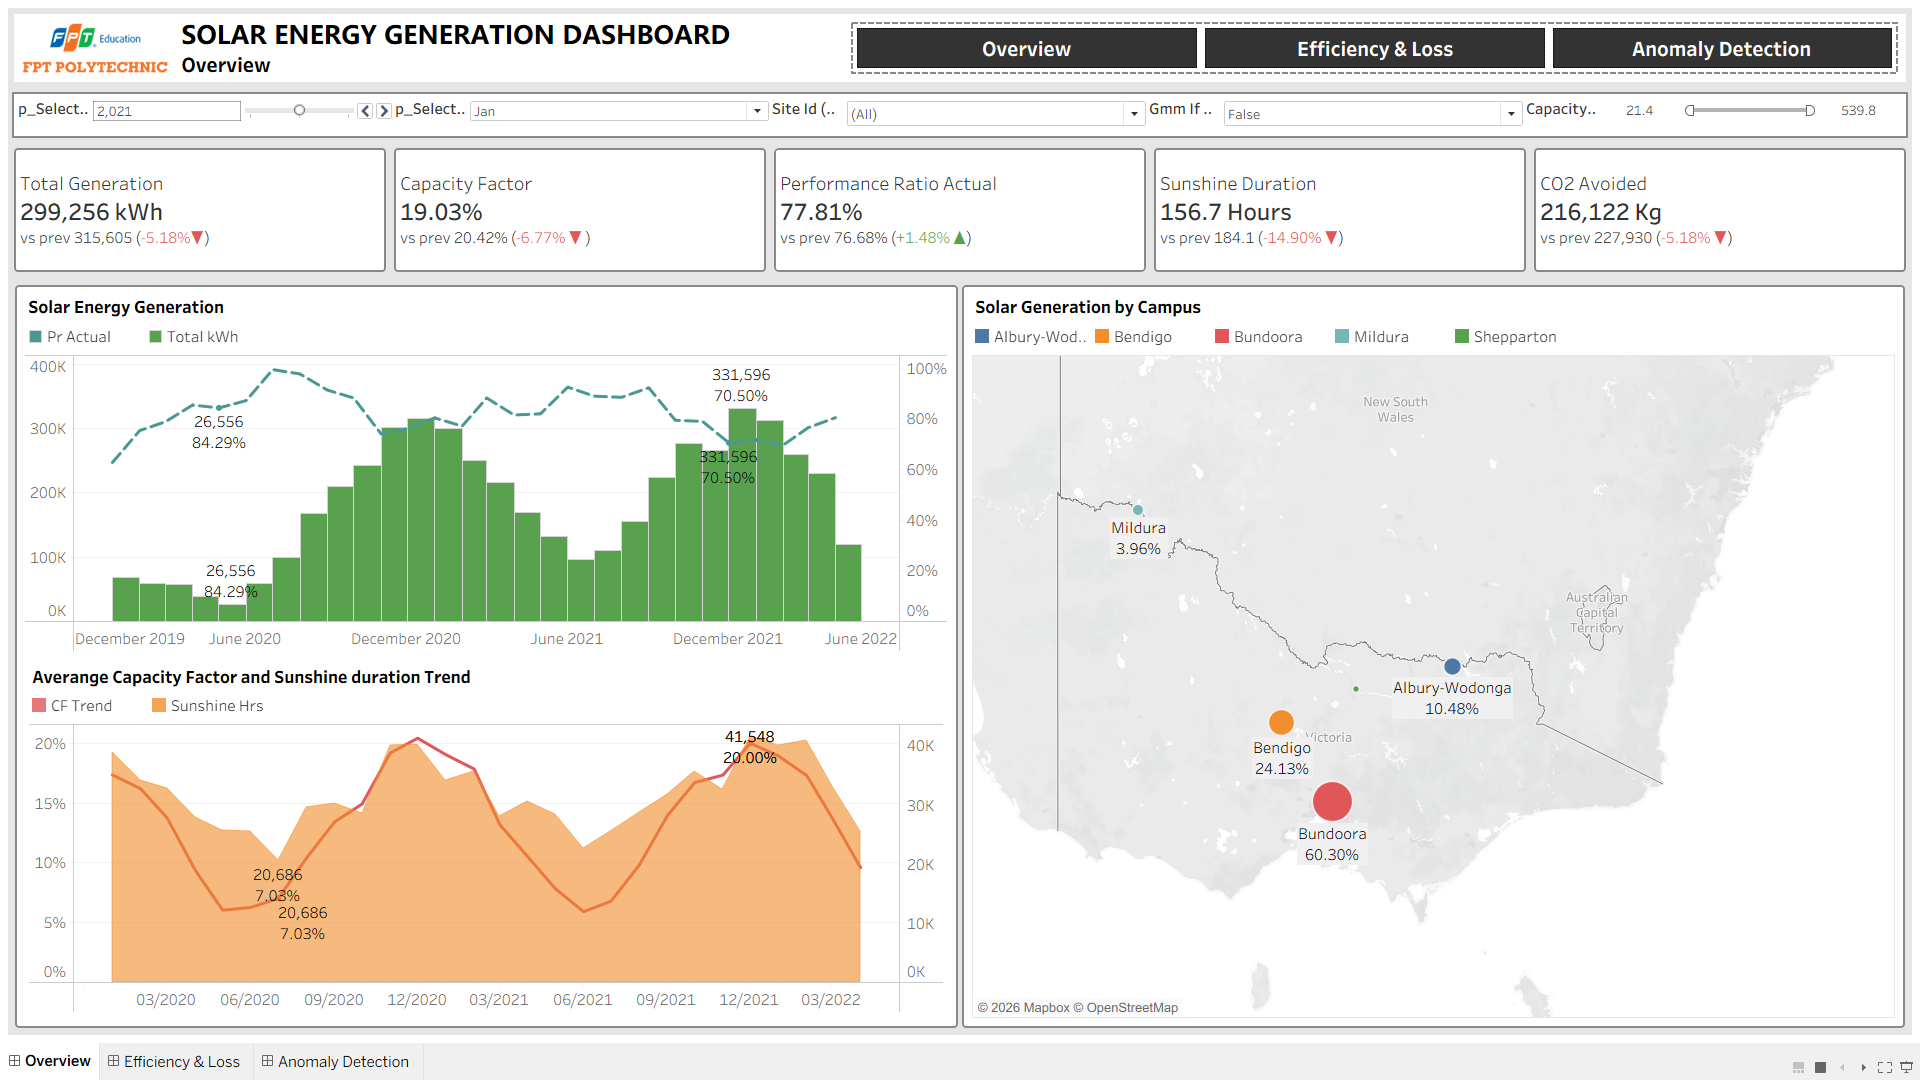
\includegraphics[width=0.95\textwidth]{figures/Dashboard_overview.png}
    \caption{Giao diện Dashboard 1: Executive Overview trên Tableau}
    \label{fig:dashboard_overview}
\end{figure}

Các thành phần giao diện và chỉ số phân tích chính bao gồm:
\begin{enumerate}[label=\alph*., leftmargin=*]
    \item \textbf{Thẻ Chỉ số Cốt lõi (BANs Layer):}
    \begin{itemize}
        \item \texttt{KPI total gen}: Hiển thị tổng sản lượng điện phát lũy kế ($E_{\text{actual}}$) tính bằng MWh/GWh, tích hợp so sánh tốc độ tăng trưởng MoM/YoY.
        \item \texttt{AVG CF}: Hệ số công suất khai thác trung bình ($\text{Capacity Factor} = \sum E / (P_{\text{stc}} \cdot 24)$).
        \item \texttt{KPI PR \& PR adjust}: Chỉ số hiệu suất thực tế ($PR_{\text{actual}}$) và chỉ số hiệu suất đã hiệu chỉnh nhiệt độ ($PR_{\text{adjusted}}$).
        \item \texttt{KPI Co2 avoided \& Sunshine dur}: Tổng khối lượng khí thải $\text{CO}_2$ triệt tiêu (kg), số cây xanh tương đương được trồng mới và tổng thời lượng nắng tích tụ trong kỳ.
    \end{itemize}

    \item \textbf{Bản đồ Địa lý Phân bố Trạm (Campus Map):}
    Trực quan hóa vị trí địa lý thực tế của 42 trạm PV tại các cơ sở đào tạo (Campus). Kích thước hình tròn (Symbol size) đại diện cho công suất thiết kế ($P_{\text{stc}}$ tính bằng $kWp$), trong khi màu sắc (Color gradient) phản ánh trực tiếp hệ số công suất CF. Nhờ đó, người quản lý lập tức nhận diện được các vùng địa lý có hiệu suất khai thác kém bất thường.

    \item \textbf{Ma trận Hiệu suất Trạm (Site Performance Matrix \& Consistency):}
    Biểu đồ xếp hạng phân bổ sản lượng ($gen/panel$) và độ ổn định vận hành giữa 42 trạm. Hệ thống trực quan hóa sự chênh lệch sản lượng trên từng tấm pin, giúp phát hiện các trạm đang hoạt động dưới mức tiềm năng thiết kế.

    \item \textbf{Xu hướng Sản lượng Tổng hợp (Total Generation \& Trend):}
    Biểu đồ đường/miền (Line/Area Chart) thể hiện sự biến đổi sản lượng theo thời gian (ngày, tháng) kết hợp phân tích đóng góp sản lượng theo từng chủng loại tấm pin (Panel Brands/Models).
\end{enumerate}

\subsection{Dashboard 2: Operational Efficiency \& Loss Analysis (Hiệu suất Vận hành \& Phân rã Tổn thất)}
\label{subsec:db_efficiency}

Dashboard \textit{Efficiency \& Loss} được thiết kế dành riêng cho đội ngũ kỹ sư kỹ thuật năng lượng nhằm ``giải thích'' nguyên nhân gốc rễ gây sụt giảm sản lượng, đặc biệt là hiện tượng suy hao do nhiệt độ (Thermal Degradation) và hiệu suất biến tần (Inverter/Optimizer).

\begin{figure}[H]
    \centering
    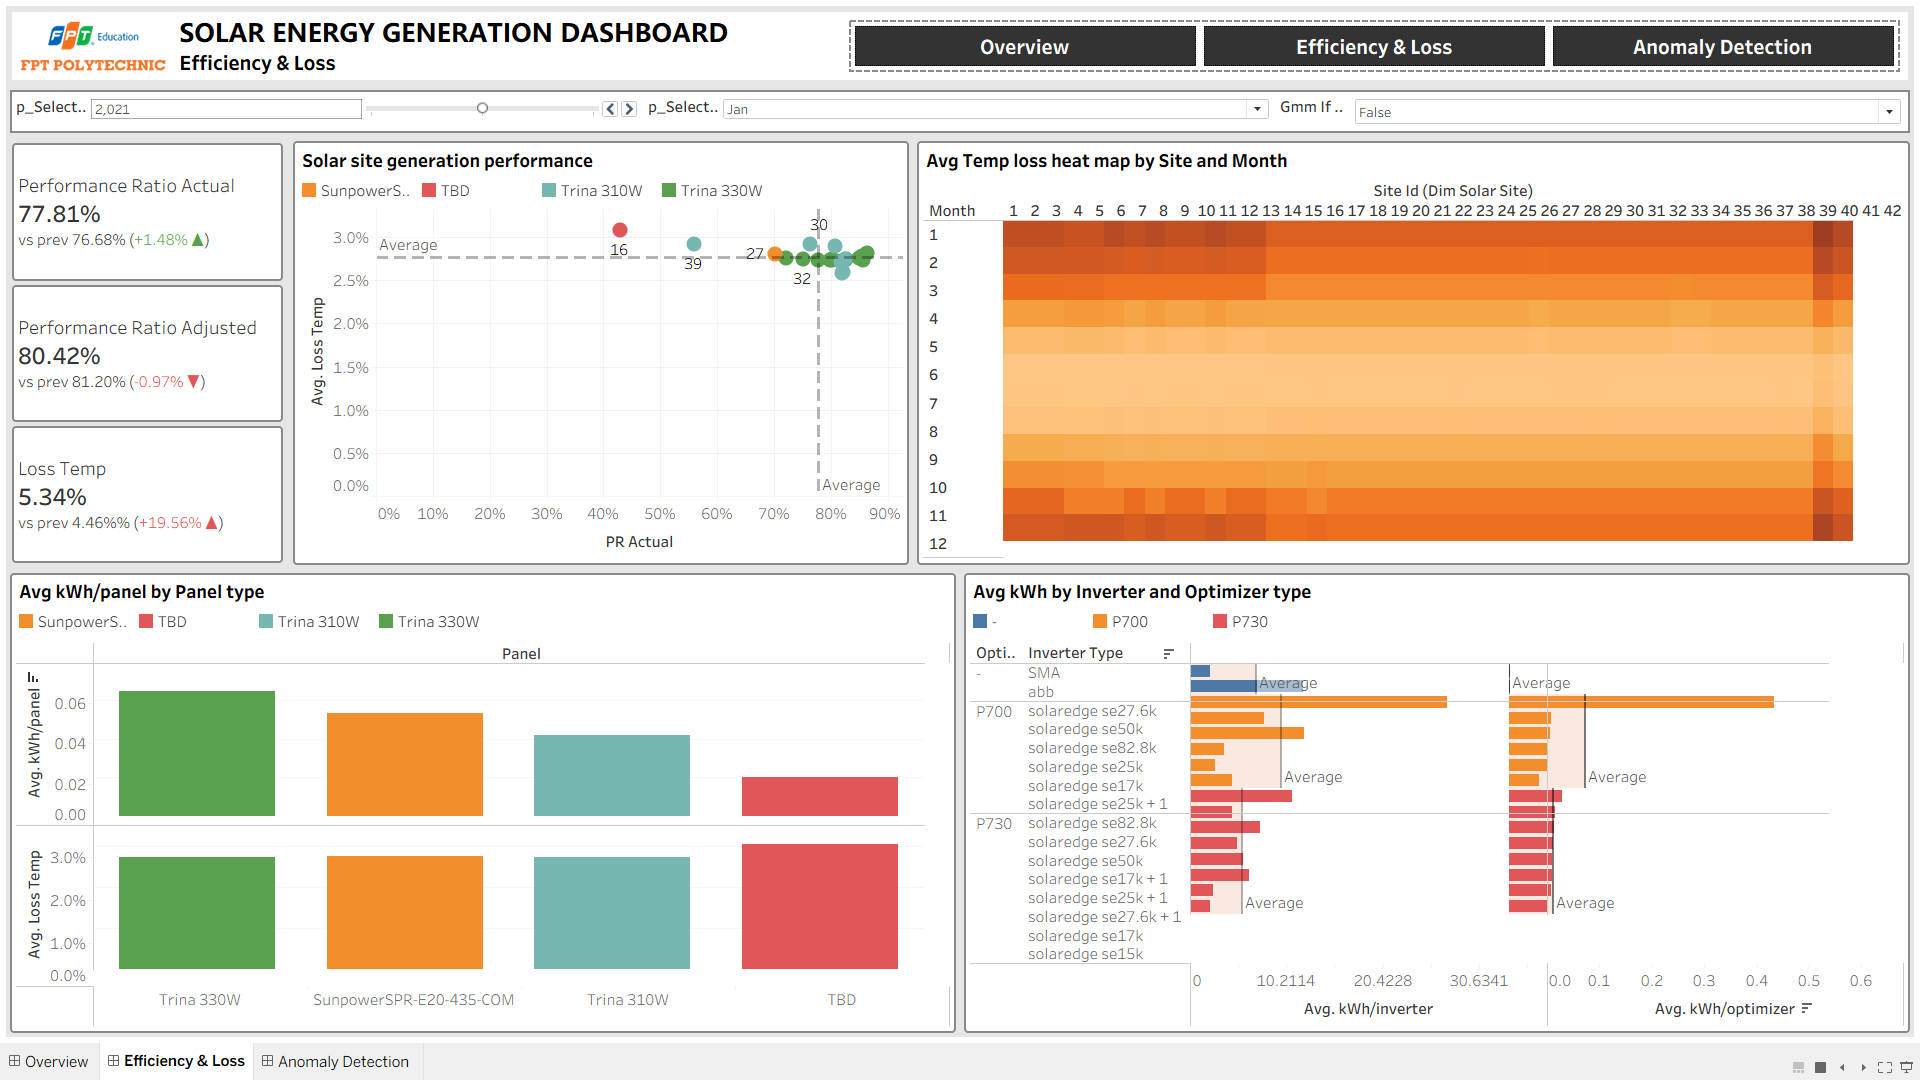
\includegraphics[width=0.95\textwidth]{figures/dashboard_efficiency_and_loss.png}
    \caption{Giao diện Dashboard 2: Operational Efficiency \& Loss Analysis trên Tableau}
    \label{fig:dashboard_efficiency}
\end{figure}

Các phân tích kỹ thuật chuyên sâu trên Dashboard bao gồm:
\begin{enumerate}[label=\alph*., leftmargin=*]
    \item \textbf{Đồ thị Xu hướng Tổn thất Nhiệt (Generation \& Loss Trend):}
    Sử dụng biểu đồ 2 trục tọa độ độc lập (Dual-Axis Chart) kết hợp giữa Sản lượng điện thực tế ($e_{\text{hourly}}$), Bức xạ sóng ngắn mặt trời (\texttt{shortwave\_radiation}) và Nhiệt độ ô pin ($T_{\text{cell}}$). Biểu đồ chứng minh luận điểm kỹ thuật quan trọng: Vào các khung giờ giữa trưa khi bức xạ đạt đỉnh cực đại ($> 800 \, \text{W/m}^2$), nhiệt độ ô pin tăng cao vượt quá $45^\circ\text{C}$ làm đường cong sản lượng bị chững lại hoặc suy giảm đáng kể so với mức lý thuyết.

    \item \textbf{Lưới Nhiệt Suy hao Nhiệt độ (Temperature Loss Heatmap \& Loss by Month):}
    Bản đồ nhiệt (Heatmap) thể hiện tỷ lệ tổn thất nhiệt độ trung bình (\texttt{avg\_loss\_temp}) phân rã theo 12 tháng trong năm và theo từng trạm phát. Dải màu chuyển từ Vàng nhạt (tổn thất $< 3\%$) sang Đỏ thẫm (tổn thất $> 8\%$), chỉ ra chính xác các tháng mùa hè đỉnh điểm cần tăng cường giải pháp làm mát hoặc thông gió bề mặt pin.

    \item \textbf{Đánh giá Hiệu suất Thiết bị (Inverter \& Optimizer Efficiency Rank):}
    Trực quan hóa chỉ số sản lượng trung bình trên mỗi tấm pin ($kWh/panel$) và tỷ lệ đáp ứng sản lượng kỳ vọng (\texttt{Yield ratio} $= E_{\text{actual}} / E_{\text{expected}}$) phân loại theo các hãng chế tạo Inverter và Optimizer. Phân tích này hỗ trợ đội ngũ bảo trì đánh giá chất lượng thiết bị vật lý thực tế để đưa ra quyết định thay thế hoặc bảo hành linh kiện.
\end{enumerate}

\subsection{Dashboard 3: Anomaly Detection \& Predictive Maintenance (Giám sát Bất thường \& Bảo trì Cảnh báo)}
\label{subsec:db_anomaly}

Dashboard \textit{Anomaly Detection} đóng vai trò là hệ thống cảnh báo sớm (Early Warning System) cho đội ngũ O\&M, trực quan hóa toàn bộ các cờ bất thường được phát hiện từ mô hình học máy GMM-IF và thuật toán Rolling IQR.

\begin{figure}[H]
    \centering
    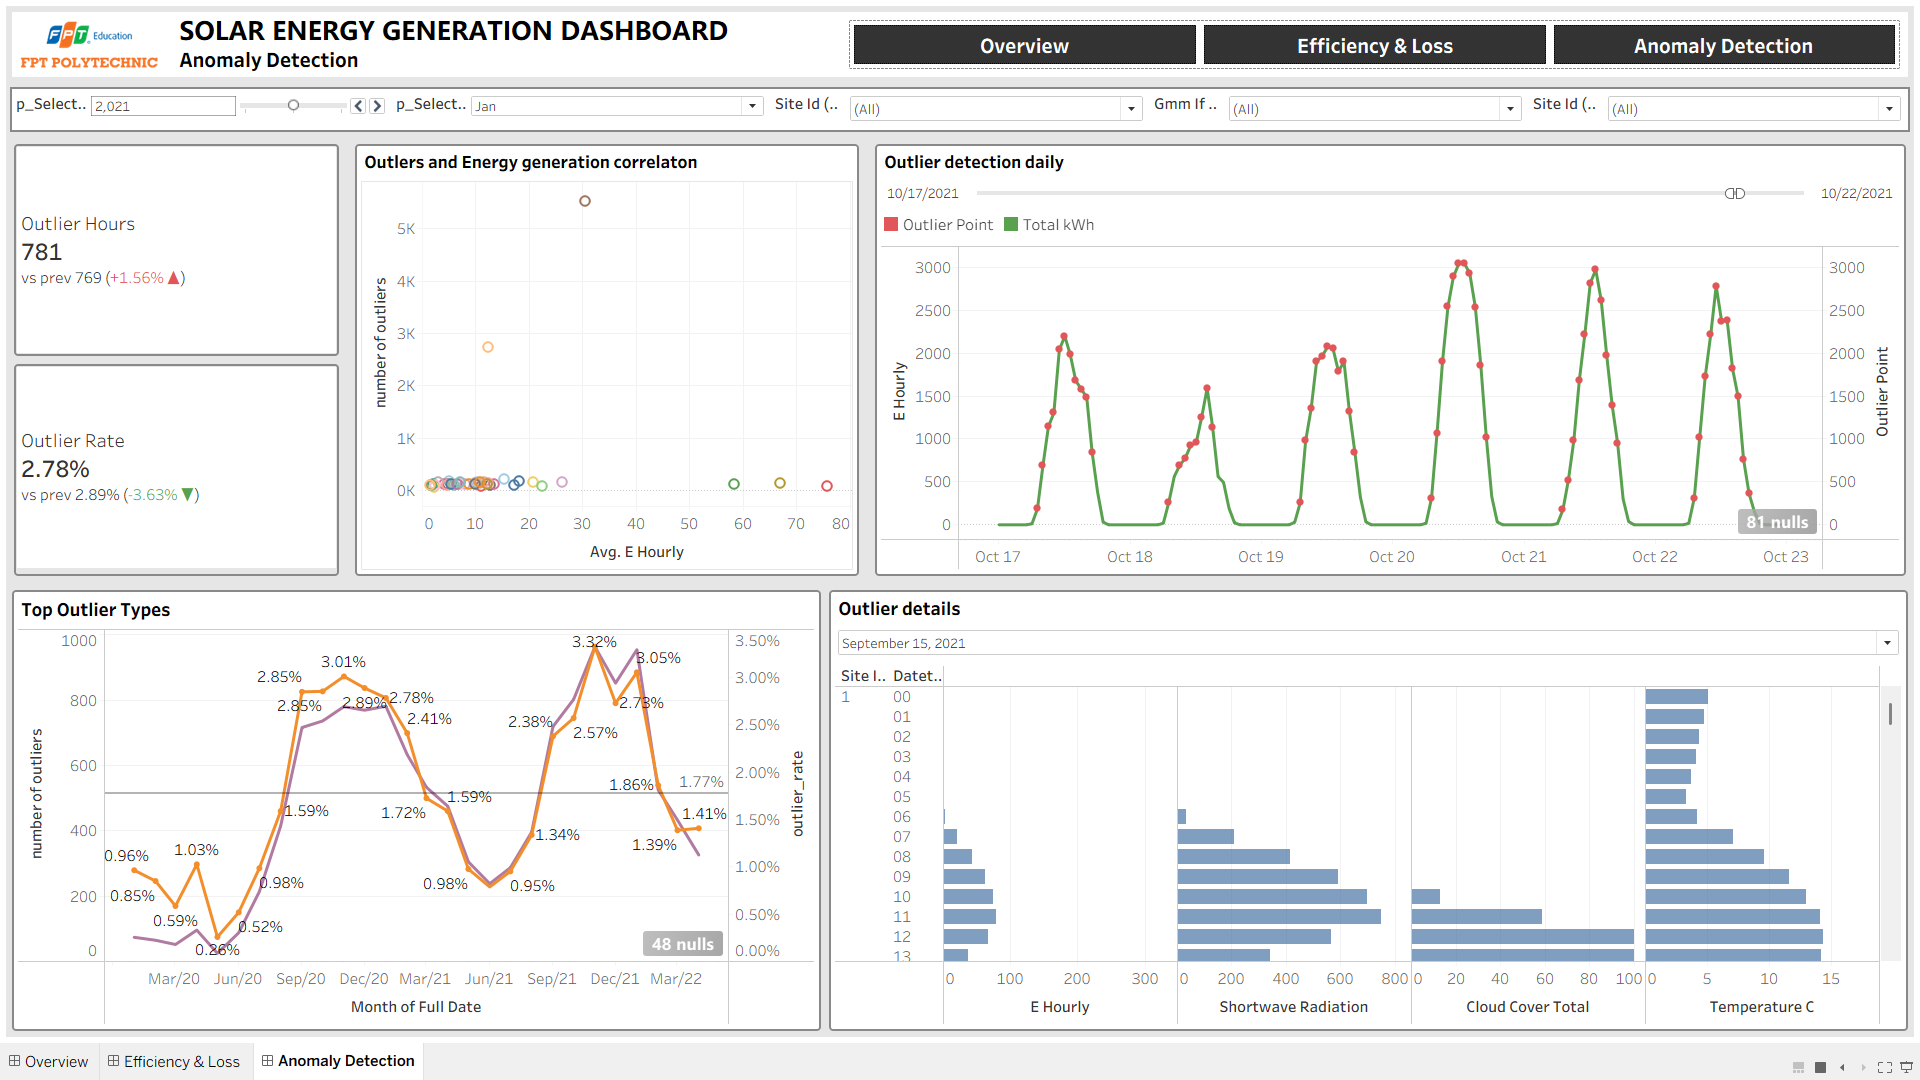
\includegraphics[width=0.95\textwidth]{figures/dashboard_anomaly_detection.png}
    \caption{Giao diện Dashboard 3: Anomaly Detection \& Predictive Maintenance trên Tableau}
    \label{fig:dashboard_anomaly}
\end{figure}

Các tính năng giám sát bất thường trọng tâm bao gồm:
\begin{enumerate}[label=\alph*., leftmargin=*]
    \item \textbf{Thẻ Thống kê Bất thường (Anomaly KPIs):}
    Hiển thị tổng số giờ phát hiện bất thường (\texttt{KPI Outlier Hours}), tỷ lệ phần trăm dữ liệu dị thường (\texttt{KPI Outlier Rate}), số lượng bản ghi gắn cờ (\texttt{number of outliers}) và chỉ số biến động so với tháng trước (\texttt{Outlier Rate MoM \%}).

    \item \textbf{Biểu đồ Chuỗi thời gian Phát hiện Dị thường (Time-series Outlier Detect):}
    Đồ thị chuỗi thời gian liên tục 15 phút biểu diễn sản lượng điện. Tất cả các mốc thời gian bị mô hình GMM-IF gắn cờ bất thường (\texttt{gmm\_if\_outlier\_flag = true}) được đánh dấu bằng các điểm nút tròn màu Đỏ rực (\texttt{\#E15759}) trên nền đường line sản lượng. Kỹ sư có thể nhấp chuột trực tiếp vào điểm dị thường để mở thẻ thông tin chi tiết (Tooltip) hiển thị lý do bất thường (\texttt{gmm\_if\_outlier\_reason}).

    \item \textbf{Bản đồ Nhiệt Phát hiện Rò rỉ Điện Ban đêm (Outlier by Site Heatmap):}
    Bản đồ nhiệt 2 chiều với Trục tung đại diện cho 24 khung giờ trong ngày ($0 - 23h$) và Trục hoành đại diện cho 42 trạm phát. 
    
    Quy tắc trực quan hóa áp đặt điều kiện đặc biệt: Nếu trong khung giờ ban đêm từ 18:30 đến 05:30 xuất hiện giá trị sản lượng $E > 0$, ô tương ứng sẽ lập tức bị tô màu Đỏ đậm. Đây là bằng chứng trực quan trực tiếp phát hiện sự cố rò rỉ dòng điện ngược (Reverse Current) hoặc cảm biến đo đạc CT bị sai lệch mốc 0 (Zero-drift fault), giúp kỹ sư khoanh vùng vị trí sự cố ngay lập tức.

    \item \textbf{Chi tiết Cảnh báo Phân loại Lỗi (Outlier Type \& Details):}
    Bảng thống kê chi tiết danh sách trạm và phân loại nhóm nguyên nhân dị thường (\textit{Night Leakage}, \textit{Extreme Power Spike}, \textit{Sensor Freeze}, \textit{Daytime Sudden Drop}), hỗ trợ lập danh mục ưu tiên cho các đội kỹ thuật đi kiểm tra hiện trường.
\end{enumerate}

% ====================================================================
%  CHƯƠNG 6: KHAI PHÁ DỮ LIỆU VÀ BUSINESS INSIGHTS
% ====================================================================
\chapter{Khai phá Dữ liệu và Dự báo Sản lượng}
\label{chap:insights}

Theo tinh thần phân tích chuyên sâu (Đừng chỉ mô tả $\rightarrow$ phải giải thích), chương này tập trung vào việc bóc tách các điểm nghẽn vận hành và đưa ra các phát hiện có giá trị kinh doanh (Business Insights) dựa trên logic dữ liệu, thay vì chỉ dựa vào các biểu đồ bề nổi. Các mô hình học máy cơ sở (ARIMA/Prophet) được tích hợp như một công cụ chẩn đoán bổ trợ.

\section{Insight 1: Hiện tượng suy giảm hiệu suất do nhiệt độ (Thermal Degradation)}
\textit{[Dữ liệu chứng minh rằng khi nhiệt độ môi trường vượt quá ngưỡng giới hạn (ví dụ: $25^\circ\text{C}$), hiệu suất chuyển đổi quang điện của tấm pin sụt giảm đáng kể. Điều này giải thích tại sao vào buổi trưa bức xạ cao nhất nhưng công suất lại không đạt đỉnh.]}

\section{Insight 2: Điểm mù vận hành từ ``Độ nhiễu ban đêm''}
\textit{[Phát hiện hàng loạt trạm ghi nhận sản lượng phát điện vào ban đêm. Nguyên nhân được phân tích là do nhiễu xung điện từ biến tần (Inverter) hoặc dòng rò. Nếu không lọc bỏ, dữ liệu này sẽ làm sai lệch nghiêm trọng các báo cáo tổng sản lượng.]}

\section{Insight 3: Ứng dụng Mô hình dự báo (Baseline) để tối ưu vận hành}
\textit{[Ứng dụng mô hình Time-Series (như Prophet) để thiết lập đường cơ sở (Baseline) dự báo sản lượng. Sự chênh lệch lớn giữa sản lượng thực tế và Baseline đóng vai trò là ``cờ báo'' (Alert) để ban quản lý cử đội bảo trì đến kiểm tra các tấm pin bị bụi bẩn bám dính hoặc hỏng hóc.]}


% ====================================================================
%  CHƯƠNG 7: KẾT LUẬN VÀ HƯỚNG PHÁT TRIỂN
% ====================================================================
\chapter{Kết luận và Hướng phát triển}
\label{chap:conclusion}

\section{Kết luận Tổng quan}
\label{sec:conclusion}
\textit{[Tóm tắt lại việc hoàn thành các mục tiêu dự án: Xây dựng thành công Data Warehouse, làm sạch dữ liệu nhiễu, và phát triển hệ thống Dashboard trực quan giúp doanh nghiệp chuyển đổi từ quản lý thụ động sang giám sát dựa trên dữ liệu.]}

\section{Khuyến nghị Chiến lược (Actionable Insights)}
\label{sec:recommendations}
\textit{[Đề xuất các hành động cụ thể: Lắp đặt hệ thống làm mát tự động để giảm suy hao nhiệt, thiết lập quy trình kiểm tra Inverter định kỳ để khắc phục độ nhiễu ban đêm, và ứng dụng kết quả dự báo để lập kế hoạch vệ sinh tấm pin.]}

\section{Hạn chế của Dự án}
\label{sec:limitations}
\textit{[Những giới hạn về phần cứng, thời gian xử lý dữ liệu lớn, hoặc sự thiếu hụt của các mô hình học sâu (Deep Learning) phức tạp hơn.]}

\section{Hướng phát triển trong tương lai}
\label{sec:future_work}
\subsection{Nâng cấp Hệ thống Phân tích Dự đoán (Predictive Analytics)}
\textit{[Tích hợp các mô hình Machine Learning mạnh mẽ hơn (XGBoost, LSTM) để dự báo biến động công suất theo thời gian thực.]}

\subsection{Tự động hóa và Đưa lên Đám mây (Cloud \& Automation)}
\textit{[Triển khai toàn bộ Pipeline ETL lên các dịch vụ Cloud như AWS/GCP để xử lý luồng dữ liệu Streaming từ các cảm biến IoT.]}

\newpage
% ====================================================================
%  PHỤ LỤC A: KẾ HẠCH THỰC HIỆN
% ====================================================================
\chapter*{Phụ lục A: Kế hoạch Thực hiện}
\addcontentsline{toc}{chapter}{Phụ lục A: Kế hoạch Thực hiện}
\label{app:kehoach}
\textit{[Bảng phân công nhiệm vụ chi tiết và kế hoạch 14 tuần thực hiện dự án của các thành viên.]}


% ====================================================================
%  PHỤ LỤC B: CẤU TRÚC MÃ NGUỒN
% ====================================================================
\chapter*{Phụ lục B: Cấu trúc Mã nguồn}
\addcontentsline{toc}{chapter}{Phụ lục B: Cấu trúc Mã nguồn}
\label{app:code}
\textit{[Sơ đồ cấu trúc thư mục của package Python du\_an\_tot\_nghiep và các script tiện ích.]}


% ====================================================================
%  TÀI LIỆU THAM KHẢO
% ====================================================================
\chapter*{Tài liệu Tham khảo}
\addcontentsline{toc}{chapter}{Tài liệu Tham khảo}
\label{chap:thamkhao}

% ====================================================================
%  TÀI LIỆU THAM KHẢO
% ====================================================================
\newpage
\begin{thebibliography}{99}
\addcontentsline{toc}{chapter}{Tài liệu Tham khảo}

% --- I. Nguồn Dữ liệu Dự án và Công trình Nghiên cứu Gốc ---
\bibitem{wimalaratne2022unisolar}
S. Wimalaratne, D. Haputhanthri, S. Kahawala, G. Gamage, D. Alahakoon và A. Jennings (2022),
``UNISOLAR: An Open Dataset of Photovoltaic Solar Energy Generation in a Large Multi-Campus University Setting'',
\textit{15th International Conference on Human System Interaction (HSI)}, IEEE, tr. 1--5.
DOI: \href{https://doi.org/10.1109/HSI55341.2022.9869474}{10.1109/HSI55341.2022.9869474}

\bibitem{openmeteo2023}
Open-Meteo GmbH (2023),
``Historical Weather API \& ERA5/ERA5-Land Reanalysis Climate Dataset''.
\url{https://open-meteo.com/en/docs/historical-weather-api}

\bibitem{iea2023pvps}
International Energy Agency (IEA) (2023),
``Photovoltaic Power Systems Programme (PVPS) Task 13: Performance, Operation and Reliability of Photovoltaic Systems'',
\textit{IEA Technical Report}.

% --- II. Thuật toán Phát hiện Bất thường và Xử lý Dữ liệu ---
\bibitem{li2025gmmif}
X. Li, G. Du, Y. Li, Z. Ma, L. Liu, M. Jiang, F. Liu và T. Mu (2025),
``Outlier Detection of Photovoltaic Power Generation System Data Based on GMM-IF Algorithm'',
\textit{IEEE Access}, tập 13, tr. 108823--108837.
DOI: \href{https://doi.org/10.1109/ACCESS.2025.3581641}{10.1109/ACCESS.2025.3581641}

\bibitem{liu2008isolation}
F. Liu, K. M. Ting và Z.-H. Zhou (2008),
``Isolation Forest'',
\textit{2008 Eighth IEEE International Conference on Data Mining}, IEEE, tr. 413--422.

\bibitem{bishop2006pattern}
C. M. Bishop (2006),
\textit{Pattern Recognition and Machine Learning (Gaussian Mixture Models)}, Springer.

\bibitem{tukey1977eda}
J. W. Tukey (1977),
\textit{Exploratory Data Analysis (IQR Rule for Outliers)}, Addison-Wesley.

\bibitem{chandola2009anomaly}
V. Chandola, A. Banerjee và V. Kumar (2009),
``Anomaly Detection: A Survey'',
\textit{ACM Computing Surveys}, tập 41, số 3, tr. 1--58.

\bibitem{kim2019missing}
T. Kim, W. Ko và J. Kim (2019),
``Analysis and Impact Evaluation of Missing Data Imputation in Day-ahead PV Generation Forecasting'',
\textit{Applied Sciences}, tập 9, số 1, bài 204.
DOI: \href{https://doi.org/10.3390/app9010204}{10.3390/app9010204}

% --- III. Mô hình Dự báo Chuỗi Thời gian và Học máy ---
\bibitem{roy2025hourly}
M. Roy, V. Pyltsov và Y. Hu (2025),
``IISE PG\&E Energy Analytics Challenge 2025: Hourly-Binned Regression Models Beat Transformers in Load Forecasting'',
Columbia University, arXiv:2505.11390.
\url{https://arxiv.org/abs/2505.11390}

\bibitem{haurwitz1945}
B. Haurwitz (1945),
``Insolation in Relation to Cloudiness and Cloud Density'',
\textit{Journal of Meteorology}, tập 2, số 3, tr. 154--166.

\bibitem{bailey2024}
M. D. Bailey và cộng sự (2024),
``Temporal and Spatial Downscaling for Solar Radiation'',
arXiv:2405.11046. \url{https://arxiv.org/abs/2405.11046}

\bibitem{engerer2014kpv}
N. A. Engerer và F. P. Mills (2014),
``KPV: A clear-sky index for photovoltaics'',
\textit{Solar Energy}, tập 105, tr. 679--693.
DOI: \href{https://doi.org/10.1016/j.solener.2014.04.019}{10.1016/j.solener.2014.04.019}

\bibitem{dev2018tes}
S. Dev, T. AlSkaif, M. Hossari, R. Godina, A. Louwen và W. van Sark (2018),
``Solar Irradiance Forecasting Using Triple Exponential Smoothing'',
\textit{IEEE International Conference on Smart Energy Systems and Technologies (SEST)}.
arXiv:1807.05872. \url{https://arxiv.org/abs/1807.05872}

\bibitem{pin2025wape}
A. Temporal-Neto và cộng sự (2025),
``PIN: A new metric to evaluate solar irradiance forecast models'',
\textit{Energy Reports}, tập 13, tr. 1--12.
DOI: \href{https://doi.org/10.1016/j.egyr.2025.01.076}{10.1016/j.egyr.2025.01.076}

\bibitem{lundberg2017shap}
S. M. Lundberg và S.-I. Lee (2017),
``A Unified Approach to Interpreting Model Predictions'',
\textit{Advances in Neural Information Processing Systems (NeurIPS)}, tập 30.
arXiv:1705.07874. \url{https://arxiv.org/abs/1705.07874}

\bibitem{zhang2013metrics}
J. Zhang, B.-M. Hodge, A. Florita, S. Lu, H. F. Hamann và V. Banunarayanan (2013),
``Metrics for Evaluating the Accuracy of Solar Power Forecasting'',
NREL/CP-5500-60142, \textit{3rd International Workshop on Integration of Solar Power into Power Systems}. OSTI Report No. 1114086.
\url{https://www.nrel.gov/docs/fy14osti/60142.pdf}

\bibitem{lonij2012tucson}
V. P. Lonij, A. E. Brooks, K. Koch và A. D. Cronin (2012),
``Analysis of 80 Rooftop PV Systems in the Tucson, AZ Area'',
\textit{38th IEEE Photovoltaic Specialists Conference (PVSC)}, tr. 549--553.
DOI: \href{https://doi.org/10.1109/PVSC.2012.6317674}{10.1109/PVSC.2012.6317674}

\bibitem{taylor2018prophet}
S. J. Taylor và B. Letham (2018),
``Forecasting at Scale (Prophet Model)'',
\textit{The American Statistician}, tập 72, số 1, tr. 37--45.

\bibitem{box2015time}
G. E. P. Box, G. M. Jenkins, G. C. Reinsel và G. M. Ljung (2015),
\textit{Time Series Analysis: Forecasting and Control}, 5th ed., John Wiley \& Sons.

\bibitem{ke2017lightgbm}
G. Ke, Q. Meng, T. Finley, T. Wang, W. Chen, W. Ma, Q. Ye và T.-Y. Liu (2017),
``LightGBM: A Highly Efficient Gradient Boosting Decision Tree'',
\textit{Advances in Neural Information Processing Systems (NeurIPS 30)}, tr. 3146--3154.

\bibitem{chen2016xgboost}
T. Chen và C. Guestrin (2016),
``XGBoost: A Scalable Tree Boosting System'',
\textit{Proceedings of KDD 2016}, ACM, tr. 785--794.

% --- IV. Kiến trúc Kho Dữ liệu, API và Công cụ Trực quan hóa ---
\bibitem{kimball2013dwh}
R. Kimball và M. Ross (2013),
\textit{The Data Warehouse Toolkit: The Definitive Guide to Dimensional Modeling}, 3rd ed., John Wiley \& Sons.

\bibitem{wmo2021guide}
World Meteorological Organization (WMO) (2021),
\textit{Guide to Meteorological Instruments and Methods of Observation (WMO-No. 8)}, WMO, Geneva, Switzerland.

\bibitem{supabase2024}
Supabase Inc. (2024),
``Supabase Open Source Enterprise PostgreSQL Data Warehouse Architecture''.
\url{https://supabase.com/docs}

\bibitem{pedregosa2011sklearn}
F. Pedregosa et al. (2011),
``Scikit-learn: Machine Learning in Python'',
\textit{Journal of Machine Learning Research}, tập 12, tr. 2825--2830.

\bibitem{tableau2023guidelines}
Tableau Software / Salesforce Inc. (2023),
``Tableau Visual Analytics \& Data Presentation Guidelines''.

\end{thebibliography}

\end{document}



